\documentclass{../mynotes}
%\usepackage[utf8]{inputenc}
\usepackage[margin=1in]{geometry}
\usepackage[usenames, dvipsnames]{xcolor}
\usepackage{graphicx}
\usepackage{mathtools}
\usepackage{amssymb}
\usepackage{amsthm}
\usepackage{fancyhdr}
\usepackage{adforn}
\usepackage{xparse}
\usepackage{tikz}
\usetikzlibrary{fadings}
%\usetikzlibrary{matrix, positioning, calc}
% Additional math macros that I want in both my notes and my psets
\usepackage[sc, noBBpl]{mathpazo}
\usepackage{mathrsfs}
\usepackage[T1]{fontenc}
\usepackage{calligra}
\usepackage{microtype}
\usepackage[all]{xy}
\usepackage{slashed}
\newcommand{\A}{\mathbb A}
\newcommand{\cat}{\mathsf}
\newcommand{\sC}{\cat C}
\newcommand{\sD}{\cat D}
\newcommand{\sS}{\cat S}
\newcommand{\sA}{\mathscr A}
\newcommand{\sF}{\mathscr F}
\newcommand{\sG}{\mathscr G}
\renewcommand{\P}{\mathbb P}
%\newcommand{\cO}{\mathscr O}
\newcommand{\cO}{\mathcal O}
\newcommand{\sI}{\mathscr I}
\DeclareMathOperator{\coker}{coker}
\renewcommand{\Im}{\operatorname{Im}}
\newcommand{\pt}{\mathrm{pt}}
\DeclareMathOperator{\Hom}{Hom}
\newcommand{\op}{^{\mathsf{op}}}
\newcommand{\Id}{\mathrm{Id}}
\DeclareMathOperator{\Mat}{Mat}
\newcommand{\m}{\mathfrak m}
%\newcommand{\p}{\mathfrak p}
\newcommand{\q}{\mathfrak q}
\newcommand{\pre}{\sC^{\text{pre}}}
\newcommand{\sh}{_{\text{sh}}}
\newcommand{\G}{\mathbb G}
\DeclareMathOperator{\Proj}{Proj}
\newcommand{\sM}{\mathscr M}
\newcommand{\sV}{\mathscr V}
\newcommand{\fU}{\mathfrak U}
\newcommand{\GL}{\mathrm{GL}}
\DeclareMathOperator{\Sym}{Sym}
% http://tex.stackexchange.com/questions/141434/how-to-type-sheaf-hom
\DeclareMathOperator{\shom}{\mathscr{H}\text{\kern -4pt {\calligra\large om}}\,}
\newcommand{\sL}{\mathscr L}
\DeclareMathOperator{\QC}{QC}
\DeclareMathOperator{\Supp}{Supp}
\newcommand{\sN}{\mathscr N}
\DeclareMathOperator{\Ann}{Ann}
\DeclareMathOperator{\Der}{Der}
\newcommand{\ctcpx}[1]{(#1)^{\text{der}}}
\newcommand{\Dist}{\mathsf{Dist}}
\newcommand{\shdi}{\operatorname{Sh}_{\Dist}}
\DeclareMathOperator{\Sh}{Sh}
\newcommand{\shz}{\mathsf{Sh}_{\text{\rm Zar}}}
\DeclareMathOperator{\Gr}{Gr}
% Source: http://tug.org/pipermail/xy-pic/2001-July/000015.html
\newcommand{\pullbackcorner}[1][dr]{\save*!/#1+1.2pc/#1:(1,-1)@^{|-}\restore}
\newcommand{\pushoutcorner}[1][dr]{\save*!/#1-1.2pc/#1:(-1,1)@^{|-}\restore}
\newcommand{\TDel}{\mathrm{2\Delta}}
\DeclareMathOperator{\Bl}{B\ell}
\newcommand{\cR}{\mathcal R}
\newcommand{\cL}{\mathcal L}
\newcommand{\cN}{\mathcal N}
\newcommand{\cH}{\mathcal H}
\newcommand{\cJ}{\mathcal J}
\newcommand{\cQ}{\mathcal Q}
\newcommand{\cZ}{\mathcal Z}
\newcommand{\cT}{\mathcal T}
\newcommand{\refR}{\reflectbox{\(\cR\)}}
\DeclareMathOperator{\ad}{ad}
\DeclareMathOperator{\Tr}{Tr}
\DeclareMathOperator{\tr}{tr}

\renewcommand{\a}{\alpha}
\renewcommand{\b}{\beta}
\newcommand{\e}{\varepsilon}
%\newcommand{\e}{\epsilon}
\renewcommand{\l}{\lambda}
\renewcommand{\L}{\Lambda}
\newcommand{\g}{\gamma}
\newcommand{\s}{\sigma}
\newcommand{\z}{\zeta}
\newcommand{\II}{\mathbb{I}}
\newcommand{\RR}{\mathbb{R}}
\newcommand{\NN}{\mathbb{N}}
\newcommand{\QQ}{\mathbb{Q}}
\newcommand{\ZZ}{\mathbb{Z}}
\newcommand{\CC}{\mathbb{C}}
\newcommand{\cB}{\mathcal{B}}
\newcommand{\cC}{\mathcal{C}}
\newcommand{\cD}{\mathcal{D}}
\newcommand{\cM}{\mathcal{M}}
\newcommand{\f}{\frac}
\newcommand{\p}{\partial}
%\renewcommand{\P}[3][]{\f{\partial^{#1} #2}{\partial #3 ^{#1}}}
\renewcommand{\P}[2]{\frac{\partial #1}{\partial #2}}
%\newcommand{\avg}[1]{\langle #1 \rangle}
\newcommand{\avg}[1]{\left< #1 \right>}
\newcommand{\?}{\overset{?}{=}}
\newcommand{\Int}{\int_{-\infty}^\infty}
%\newcommand{\ket}[1]{\left| #1 \right>} % for Dirac bras
%\newcommand{\bra}[1]{\left< #1 \right|} % for Dirac kets
%\newcommand{\braket}[2]{\left< #1 \vphantom{#2} \right|
% \left. #2 \vphantom{#1} \right>} % for Dirac brackets
\DeclarePairedDelimiter\bra{\langle}{\rvert}
\DeclarePairedDelimiter\ket{\lvert}{\rangle}
\DeclarePairedDelimiterX\braket[2]{\langle}{\rangle}{#1 \delimsize\vert #2}
\newcommand{\kb}[2]{\left\lvert #1 \middle\rangle\!\middle\langle #2 \right\rvert}
\newcommand{\dyad}[1]{\left\lvert{#1}\middle\rangle\!\middle\langle{#1}\right\rvert}%{\left| #1 \right>\left< #1 \right|}
\DeclarePairedDelimiter{\ceil}{\lceil}{\rceil}
\newcommand{\ul}[1]{\underline{#1}}
\def\normord#1{\mathop{:}\nolimits\!#1\!\mathop{:}\nolimits}
%\newcommand{\normord}[1]{{:}\!\mathrel{#1}\!{:}}

%vector calculus
\newcommand{\grad}[1]{\gv{\nabla} #1} % for gradient
\let\divsymb=\div % rename builtin command \div to \divsymb
\renewcommand{\div}[1]{\gv{\nabla} \cdot #1} % for divergence
\newcommand{\curl}[1]{\gv{\nabla} \times #1} % for curl

%lists are (a) (b) (c) by default
\renewcommand{\labelenumi}{(\alph{enumi})}

\newcommand{\term}{\emph}

%vectors
\renewcommand{\vec}[1]{\boldsymbol{\mathbf{#1}}}
\let\vaccent=\v % rename builtin command \v{} to \vaccent{}
\renewcommand{\v}[1]{\ensuremath{\mathbf{#1}}}
\newcommand{\uv}[1]{\ensuremath{\mathbf{\hat{#1}}}} % for unit vector
\newcommand{\gv}[1]{\ensuremath{\mbox{\boldmath$ #1 $}}} 
% for vectors of Greek letters

%\usepackage[framemethod=TikZ]{mdframed}
%\newenvironment{framedefn}[2][]{
%    \stepcounter{equation}
%    \begin{mdframed}[frametitle={Definition}]\relax%
%    \label{#2}
%}{\end{mdframed}}
\usepackage{hyperref}
\usepackage{siunitx}

%\usepackage[compat=1.1.0]{tikz-feynman}

% TODO fiddle with colors
\definecolor{newblue}{HTML}{1F98A6}
\definecolor{newred}{HTML}{D95448}
\definecolor{neworange}{HTML}{F29441}
\hypersetup{
	colorlinks,
	linkcolor=newred,
	citecolor=neworange,
	urlcolor=newblue!80!black,
}
\usepackage[all]{hypcap}
\pagestyle{plain}
\setcounter{tocdepth}{1}


\usepackage{titlesec}
\titleformat{\section}[frame]
  {\normalfont}
  {\filright
   \footnotesize
   \enspace Lecture \arabic{section}.\enspace}
  {8pt}
  {\Large\bfseries\filcenter}
\usepackage[dotinlabels]{titletoc}
\titlecontents{section}[1.5em]{}{\contentslabel{2.3em}}{\hspace*{-2.3em}}{\hfill\contentspage}

\renewcommand{\sectionmark}[1]{\markleft\thesection. #1}

\fancyhf{}
\fancyhead[RO,LE]{\small\thepage}
\fancyhead[LO]{\small\slshape\nouppercase{\rightmark}}
\setlength{\headheight}{11.0pt}
\pagestyle{fancy}

\numberwithin{equation}{section}
\newcommand{\orbreak}{
\begin{center}
	\adforn{17}\;\(\cdot\)\;\adforn{18}
	\vspace{0.2cm}
\end{center}
}

\renewcommand{\labelitemi}{\(\circ\)}

% I wanted to allow one to reference parts of a thm/cor/etc. and have it print the thm number too, e.g. 29.2(1),
% but this isn't working right now. Probably the best way to do this would be to play around with enumitem to
% define a new enumerate-like counter and then just use that directly instead of enumerate in comp.

% This feels really wobbly, but so far it's working
\NewDocumentEnvironment{comp}{mm}{%
	\csname #1\endcsname\hfill
	\csname #2\endcsname
}{
	\csname end#2\endcsname
	\csname end#1\endcsname
}

% usage:
% \shortexact[f][g]{A}{B}{C},
%
%			 f    g
% for 0 -> A -> B -> C -> 0,
\DeclareDocumentCommand{\shortexact}{O{} O{} mmmm}{
\xymatrix{
	0\ar[r] & #3\ar[r]^-{#1} & #4\ar[r]^-{#2} & #5\ar[r] & 0#6
}}
% exactly the same, but for 0 -> A -> B -> C
\DeclareDocumentCommand{\leftexact}{O{} O{} mmmm}{
\xymatrix{
	0\ar[r] & #3\ar[r]^-{#1} & #4\ar[r]^-{#2} & #5 #6
}}
% ... and the same, for A -> B -> C -> 0
\DeclareDocumentCommand{\rightexact}{O{} O{} mmmm}{
\xymatrix{
	#3\ar[r]^-{#1} & #4\ar[r]^-{#2} & #5\ar[r] & 0#6
}}



% usage:
% X\dblarrow[r] & Y
%   f
% X => Y
%   g
\DeclareDocumentCommand{\dblarrow}{O{} O{} O{}}{
	\ar@<0.4ex>[#1]^-{#2}\ar@<-0.4ex>[#1]_-{#3}
}
% Note: it would be a useful exercise to figure out how to define this so it can be used as
% \dblarrow[r]^f_g

\everyentry={\displaystyle}

\DeclarePairedDelimiter\paren{(}{)}
%\DeclarePairedDelimiter\ang{\langle}{\rangle}
\DeclarePairedDelimiter\abs{\lvert}{\rvert}
\DeclarePairedDelimiter\norm{\lVert}{\rVert}
\DeclarePairedDelimiter\bkt{[}{]}
\DeclarePairedDelimiter\set{\{}{\}}
% Swap paren* and paren, etc., so that the normal version resizes by default.
% Meanwhile, one can use \paren*[\Big]{...} to customize the size easily.
% It would be interesting to wrap this up into a custom \definedelimiter command...
\makeatletter
	\let\oldparen\paren
	\def\paren{\@ifstar{\oldparen}{\oldparen*}}
	\let\oldbkt\bkt
	\def\bkt{\@ifstar{\oldbkt}{\oldbkt*}}
\makeatother
\def\qedsymbol{{\small{\ensuremath{\boxtimes}}}}
\newcommand{\inj}{\hookrightarrow}
\newcommand{\surj}{\twoheadrightarrow}
\DeclareMathOperator{\id}{id}
\newcommand{\ud}{\,\mathrm{d}}
\renewcommand{\d}{\mathrm d}
\newcommand{\dfr}[2]{\frac{\mathrm d #1}{\mathrm d #2}}
\newcommand{\pfr}[2]{\frac{\partial #1}{\partial #2}}

%\catcode`\"=13
%\newcommand{"}[1]{^{(#1)}}
\newtheorem{thm}[equation]{Theorem}
\newtheorem*{thm*}{Theorem}
\newtheorem{lem}[equation]{Lemma}
\newtheorem*{lem*}{Lemma}
\newtheorem{cor}[equation]{Corollary}
\newtheorem{prop}[equation]{Proposition}
\newtheorem{obs}[equation]{Observation}
\theoremstyle{definition}
\newtheorem{ex}[equation]{Exercise}
\newtheorem{exm}[equation]{Example}
\newtheorem{defn}[equation]{Definition}
\newtheorem*{claim}{Claim}
\theoremstyle{remark}
\newtheorem*{rem}{Remark}
\newtheorem*{fct}{Fact}
\newtheorem*{note}{Note}

\begin{document}
\title{Physics 200B: Electromagnetism I}
\author{Ian Lim\\ Last updated \today}
\fancyhead[RE]{\small\slshape Physics 200B Lecture Notes}
\maketitle
{\small\noindent These notes were taken for Physics 200B, \emph{Electromagnetism I}, as taught by Rena Zieve at the University of California, Davis in winter quarter 2020. I live-\TeX ed them using Overleaf, and as such there may be typos; please send questions, comments, complaints, and corrections to 
\href{mailto:itlim@ucdavis.edu?subject=200B\%20Lecture\%20Notes}{\texttt{itlim@ucdavis.edu}}.\\
Many thanks to Arun Debray for the {\LaTeX} template for these lecture notes: as of the time of writing, you can find him at \url{https://web.ma.utexas.edu/users/a.debray/}.}

\tableofcontents

%week 1
\section{Tuesday, January 7, 2020}
	Here's some filler text.
\section{Thursday, January 9, 2020}
    Today we'll start our discussion with Gauss's law, moving rapidly into chapter 3 of Zangwill. Gauss's law lets us calculate electric fields rapidly for situations with high amounts of symmetry. Basically, we can solve systems with spherical symmetry, cylindrical symmetry, and translational plane symmetry. It doesn't get us too far but it's a lot better than Coulomb's law volume integrals.

As we know, Gauss's law (differential form) states
\begin{equation}
    \div \vec E = \frac{\rho}{\epsilon_0},
\end{equation}
or in integral form
\begin{equation}
    \oint_S \vec E \cdot d\vec A = \int_V \div \vec E d^3 r = \int_V \frac{\rho}{\epsilon_0} d^3 r = \frac{Q_\text{enc}}{\epsilon_0}.
\end{equation}
The simplest example is for the point charge. For a single positive charge $q>0$, we can reason that the field must point in the radial direction and it is constant at surfaces of constant $R$, so that $\vec E(r,\theta,\phi) = E(r) \uv r$. Then
\begin{equation}
    \oint_S \vec E \cdot d\vec A = |E| 4\pi R^2 = \frac{q}{\epsilon_0},
\end{equation}
which yields
\begin{equation}
    \vec{E} = \frac{q}{4\pi R^2 \epsilon_0} \uv r.
\end{equation}
Gauss's law also gives us a nice result (sometimes known as Newton's shell theorem), which says that the electric field due to a spherically symmetric shell of charge \emph{inside} that shell ($r<R$) is zero.

We can also do Gauss's law for an infinite plane by drawing a Gaussian pillbox, say, extending a height $h$ above and below the plane. Rotational symmetry lets us reason that the field can only point in the normal direction to the plane, while reflection symmetry says its magnitude is the same equal distances above and below the plane. It follows that
\begin{equation}
    \oint_S \vec E \cdot d \vec A = \frac{1}{\epsilon_0} \sigma A,
\end{equation}
where $A$ is the area of the face of the Gaussian pillbox. Since the field is normal to the plane and the faces of the pillbox are oriented outwards, we have
\begin{equation}
    \oint_S \vec E \cdot d\vec A = 2 E(h) A,
\end{equation}
so that
\begin{equation}
    \vec{E}(h) =\begin{cases}
        \frac{\sigma}{2\epsilon_0}\uv z & z >0\\
        -\frac{\sigma}{2\epsilon_0} \uv z & z < 0.
    \end{cases}
\end{equation}
The reason there is no $h$ dependence is because the infinite plane is scale-invariant. If we rescale all the coordinates, the infinite plane still looks like an infinite plane. This result isn't necessarily useful to us because real life is filled with infinite planes of charge, or even because the problem is exactly solvable; rather, it's because any reasonably smooth (in the mathematical sense) surface looks locally flat, which means that near the surface, we have essentially the field from an infinite plane. 

By the same Gaussian pillbox arguments, we find that $E_\parallel$ is continuous at surfaces of charge, while $E_\perp$ is discontinuous by $\frac{\sigma}{\epsilon_0}$.
How should we calculate the force on a little surface of charge, given that the electric field is discontinuous above and below the field? Well, we can just take the average. This seems physically reasonable, but we can justify it. Remember the discontinuity comes from the charge at the surface itself, and as we showed last time, charges cannot exert forces on themselves. So if we average above and below the surface, we will basically average away the contribution of the charged surface itself and get the right answer.
%figure

We can also state Earnshaw's theorem-- in a closed region with no charge, any extrema of the potential must be on the boundary. For suppose there was a local maximum of the potential in the interior. The gradient of the potential vanishes at that point, and a little bit away we can draw a Gaussian surface it is pointing towards that point everywhere. %figure
It follows that the $\vec E$-field points away everywhere, so our integral $\oint_S \vec E \cdot d\vec A > 0$, which violates our assumption that there was no charge in the region.%
    \footnote{One can also argue this directly from the form of Laplace's equation.}
This tells us that we cannot make an electrostatic cage; no charge distribution can hold itself in a static configuration under Coulomb interactions alone. Earnshaw's theorem has told us that any charge dropped in a region with no other charge will move to the edges of that region, since it cannot sit at an extremum.

\subsection*{Potential and potential energy}
For our purposes, we will follow Zangwill and denote potential energy by $V$ and electrostatic potential by $\varphi$. We say the potential energy changes as
\begin{equation}
    \delta V = -\vec F \cdot d\vec s
\end{equation}
for small displacements, i.e.
\begin{equation}
    \vec F = -\grad V.
\end{equation}
In addition, when forces are due only to electric fields, then
\begin{equation}
    \vec F = q\vec E = -q \grad \varphi \implies V = q\varphi.
\end{equation}
Hence the electrostatic potential is the energy per charge.

Let's now prove \term{Green's reciprocity relation} for the potential energy. That is, suppose there are two charge distributions $\rho_1,\rho_2$. The energy of $\rho_2$ in the potential $\varphi_1$ created by $\rho_1$ is
\begin{equation}
    V = \int d^3 r \, \rho_2(\vec r) \varphi_1(\vec r),
\end{equation}
such that
\begin{equation}
    \delta V = \int d^3 r \, \bkt{\rho_2(\vec r-\delta \vec s)-\rho_2(\vec r)} \varphi_1(\vec r).
\end{equation}
The minus sign comes from that active/passive transformation jazz. If the distribution is moved by $\delta \vec s$, then looking at the ``same'' point in space $\vec r$ for the new distribution is equivalent to looking at the original distribution at a point $\vec r - \delta \vec s$.

We can now Taylor expand as $\delta \vec s$ gets small, such that
\begin{equation}
    \delta V \approx - \delta \vec s \cdot \int d^3 r \, (\grad \rho_2(\vec r)) \varphi_1(\vec r) = -\delta\vec s \cdot \int d^3 r\paren{\grad(\rho_2 \varphi_1) - \rho_2 \grad \varphi_1},
\end{equation}
after a product rule manipulation (basically an integration by parts). Now this first term is a total derivative, so it vanishes as we take our integration region $d^3r$ to be all space. What's left is
\begin{equation}
    \delta V = -\delta \vec s \cdot \int d^3 r \, \rho_2(\vec r) \vec E_1(\vec r).
\end{equation}

Let us rewrite this energy in a different way:
\begin{equation}
    V = \int d^3 r \, \rho_2(\vec r) \varphi_1(\vec r) = \frac{1}{4\pi \epsilon_0} \int d^3 r \int d^3 r' \, \rho_2 (\vec r) \frac{\rho_1(\vec r')}{|\vec r - \vec r'|}.
\end{equation}
But notice that this integral is manifestly symmetric in $\vec r$ and $\vec r'$ (i.e. $|\vec r- \vec r'| = |\vec r' - \vec r|$). This certainly converges, so we can switch the order of integration and do the $d^3 r$ integral first to find
\begin{equation}
    V = \int d^3 r \, \rho_2(\vec r) \varphi_1(\vec r) = \int d^3 r' \, \rho_1(\vec r') \varphi_2(\vec r').
\end{equation}
This relation means that the energy in an electrostatic charge distribution doesn't depend on how we build it, only on the final geometry.

Consider the following example.
\begin{exm}
    Suppose we have a spherical region of radius $R$ centered on the origin with no charge inside. As it turns out, the potential at the center is the average potential on the surface:%
        \footnote{Again, this is a property of Laplace's equation. For a good reference on this, see Evans \textit{Partial Differential Equations}, section 2.2.2.}
    \begin{equation}
        \varphi(0) = \frac{1}{4\pi R^2} \int dS \varphi(\vec r).
    \end{equation}
    Can we use Green's reciprocity relation to find this result? Take 
    \begin{equation}
        \varphi_1 = \varphi, \quad \rho_1 = \rho; \quad \rho_2(\vec r) = \frac{q}{4\pi R^2} \delta(r-R).
    \end{equation}
    Then
    \begin{equation}
        \varphi_2 = \begin{cases}
            \frac{q}{4\pi \epsilon_0 r} & r \geq R,\\
            \frac{q}{4\pi \epsilon_0 R} & r \leq R.
        \end{cases}
    \end{equation}
    It follows that
    \begin{equation}
        \int d^3 r \frac{q}{4\pi R^2} \delta(r-R) \varphi(\vec r) = \int d^3r \rho(\vec r) \varphi_2(\vec r) = \int_R^\infty r^2 dr \int d\Omega \rho(\vec r) \frac{q}{4\pi \epsilon_0 r}.
    \end{equation}
    But this last expression up the the factor of $q$ is exactly the integral we would use to compute the potential at the origin. That is,
    \begin{equation}
        \int_R^\infty r^2 dr \int d\Omega \rho(\vec r) \frac{q}{4\pi \epsilon_0 r} = q \varphi(\vec r=0).
    \end{equation}
    Meanwhile, the LHS says that we just integrate
    \begin{equation}
        \int d^3 r \frac{q}{4\pi R^2} \delta(r-R) \varphi(\vec r) = \frac{q}{4\pi R^2} \int dS \,\varphi(\vec r).
    \end{equation}
    Cancelling the factors of $q$, we have exactly the desired result. The potential at the center of the sphere is equal to the average potential on its surface.
\end{exm}

We can write the potential energy of a charge distribution as
\begin{equation}
    U_E = \frac{1}{4\pi \epsilon_0} \sum_{j=1}^N \sum_{i>j}^N \frac{q_i q_j}{|\vec r_i - \vec r_j|}
\end{equation}
or for continuous distributions,
\begin{equation}
    U_E = \frac{1}{8\pi \epsilon_0} \int d^3 r \int d^3 r' \frac{\rho(\vec r) \rho(\vec r')}{|\vec r - \vec r'|} = \frac{1}{2} \int d^3 r \rho(\vec r) \varphi(\vec r)
\end{equation}
Note that for all-positive or all-negative distributions of charges, these formulae make it clear that the energy of assembling the distribution is positive-definite. The answer is somewhat less clear when we have a mix of charges. Let's manipulate this result to see what happens.
\begin{align*}
    U_E &= \frac{1}{2} \int d^3 r \rho(\vec r) \varphi(\vec r)\\
        &= \frac{1}{2} \int d^3r \epsilon_0 \div \vec E \varphi(\vec r)\\
        &= \frac{\epsilon_0}{2} \int d^3 r \paren{\div(\vec E \varphi) - \vec E \cdot (\grad \phi)}\\
        &\to \frac{\epsilon_0}{2} \int d^3 r |E|^2
\end{align*}
where the last step is taking the limit as the region of integration becomes all space, and the total derivative term goes away. 

So $U_E$ for continuous distributions defined in this way is \emph{positive-definite}. How does this square with our idea that we could just bring one positive and one negative charge together? Well, it takes energy to assemble the charges in the first place. In fact, one can check that the energy of a point charge is divergent since it's a finite amount of charge squished into a single point of space. Part of the energy in this expression (summing up the energy in the E-field) comes from actually assembling the charge distribution, and we'll get some practice with this on the homework.
    
%week 2
\section{Tuesday, January 14, 2020}
    \subsection*{Multipole expansion}
Today we're moving into Chapter 4 of Zangwill, on multipoles. Multipoles are a way of thinking about the field of a charge distribution far away from that distribution. For instance, if there is a net charge in that distribution, far away we have a field that decays as $1/r^2$, like the field of a point charge.

Suppose we have a charge distribution $\rho(\vec r')$ contained entirely within a sphere of radius $R$. That is, $\rho(\vec r') =0$ for $|\vec r'| > R$. Then we can look at a point $\vec r$ outside the sphere with $|\vec r| > R$. Well, our potential is just given by
\begin{equation}
    \varphi(\vec r) = \frac{1}{4\pi \epsilon_0} \int d^3 r' \frac{\rho(\vec r')}{|\vec r-  \vec r'|},
\end{equation}
and we'd like to expand the denominator when $|\vec r| \gg |\vec r'|$. Our expansion looks like
\begin{equation}
    \frac{1}{|\vec r- \vec r'|} \approx \frac{1}{r} - \vec r' \cdot \grad \frac{1}{r} + \frac{1}{2}(\vec r' \cdot \grad)^2 \frac{1}{r} - \dots
\end{equation}
If we're being careful we should really expand in $r'/r$ as a small parameter. The derivatives are all with respect to unprimed coordinates, and then the $\vec r'$ determines which direction we're looking. This is much better in index notation. With the Einstein summation convention (i.e. sum over repeated indices), this becomes
\begin{equation}
    \frac{1}{|\vec r- \vec r'|} \approx \frac{1}{r} - r_i' \grad_i \frac{1}{r} + \frac{1}{2} r_i' r_j' \grad_i \grad_j \frac{1}{r}+ \dots
\end{equation}
If we plug this expansion back into the expression for the potential, we get
\begin{equation}
    \varphi(\vec r) = \frac{1}{4\pi \epsilon_0} \set*{\underbrace{\bkt{\int d^3 r' \rho(\vec r')}}_{\text{monopole}=Q} \frac{1}{r} - \underbrace{\bkt{\int d^3 r' \rho(\vec r') r_i'}}_{\text{dipole}=\vec p} \p_i \frac{1}{r}+ \underbrace{\bkt{\frac{1}{2} \int d^3 r' \rho(\vec r') r_i' r_j'}}_{\text{quadrupole}=Q_{ij}} \grad_i \grad_j \frac{1}{r} + \dots}
\end{equation}

A note on tensors. Tensors are like collections of numbers that have special properties under coordinate transformations. A rank 1 tensor is just a vector; we need only one number to label which component we are looking at. So if we write a vector $\vec v = (a,b,c)$ then we can also write its components $v_i$ such that $v_1=a,v_2=b,v_3=c$. 

Similarly matrices are rank two tensors--- we need two index labels to say which element we are looking at. That is, a $3\times 3$ matrix requires two index labels to pick out an element, a row and a column. We can guess what a rank three tensor looks like, i.e. some sort of cube of numbers. After rank three it's best to just think of these in the abstract. However, not any collection of numbers is a tensor. Each row and column of a matrix must transform like a vector.

Note that many of the complications of working with tensors (e.g. where do you put the indices, up or down?) will drop out when we work in flat Cartesian coordinates.

Can we study the limiting behavior of this expansions? Sure, if we perform some dimensional analysis. We took our charge to be confined to a sphere of radius $R$; the monopole moment is independent of $R$, while the dipole and quadrupole components scale as
\begin{equation}
    p_i \sim QR, \quad Q_{ij} \sim QR^2.
\end{equation}
Derivatives with respect to the $\vec r$ unprimed coordinates act like $1/r$, so our approximation looks like
\begin{equation}
    \varphi(r) \sim \frac{1}{4\pi \epsilon_0} \bkt{\frac{Q}{r} - \frac{QR}{r^2} + \frac{QR^2}{r^3} + \dots}.
\end{equation}
If we work out the derivatives, we get
\begin{equation}
    \varphi(\vec r) = \frac{1}{4\pi \epsilon_0} \set*{\frac{Q}{r} + \frac{p_i r_i}{r^3} + Q_{ij} \frac{3r_i r_j - r^2 \delta_{ij}}{r^5}+ \dots}
\end{equation}

Let us find the field of the dipole term far away.
\begin{align}
    \vec E &= - \grad \varphi_\text{dipole}\\
        &=-\frac{1}{4\pi \epsilon_0} \grad \paren{\frac{\vec p \cdot \vec r}{r^3}}.
\end{align}
We will write this vector in terms of its components. Note that $\p_i r= \p_i \sqrt{x^2 +y^2+z^2} = \frac{r_i}{\sqrt{x^2+y^2+z^2}} = r_i/r$. Then
\begin{align*}
    E_i &= - \frac{1}{4\pi \epsilon_0} \p_i \paren{\frac{p_j r_j}{r^3}}\\
        &= -\frac{1}{4\pi \epsilon_0} \bkt{p_j \frac{\delta_{ij}}{r^3} - \frac{3 p_j r_j}{r^4} \p_i r }\\
        &= -\frac{1}{4\pi \epsilon_0} \bkt{p_j \frac{\delta_{ij}}{r^3} - \frac{3 p_j r_j r_i}{r^5}}\\
        &= \frac{1}{4\pi \epsilon_0} \bkt{ \frac{\vec p \cdot \vec r}{r^5} r_i - \frac{p_i}{r^3}}.
\end{align*}
Equating these as vectors gives
\begin{equation}
    \vec E = \frac{1}{4\pi \epsilon_0} \bkt{\frac{3 \vec p \cdot \uv r}{r^3} \uv r - \frac{\vec p }{r^3}}.
\end{equation}

One can model a physical dipole as two charges, one $+q$ and one $-q$, separated by a distance $a$ and connected by a rigid ``rod'' of some sort. Then the dipole moment is $q\vec a$. One can imagine shrinking this dipole down by keeping the product $qa$ fixed while taking $a\to 0$. In a sense, a dipole is like a derivative of a delta function.

In constant electric fields, there is no net force on a dipole since each of the charges experiences an equal and opposite force. (In general there will be a torque.) It's only when the field is changing that we experience a net force, so we may think of dipoles as sensitive to gradients in the field.

\subsection*{The quadrupole}
The quadrupole moment was defined as
\begin{equation}
    Q_{ij} = \frac{1}{2} \int d^3 r'(\rho (\vec r') r_i' r_j',
\end{equation}
and from this expression we see that $Q_{ij} = Q_{ji}$, e.g. $Q_{12}=Q_{21}$, and so on. It is symmetric, and hence in 3 dimensions there are 6 independent components. If we choose our axes really well, we can diagonalize the quadrupole tensor and just compute three components.

We can also define the \term{traceless quadrupole tensor} as
\begin{equation}
    \Theta_{ij} = 3 Q_{ij} - Q_{kk} \delta_{ij}.
\end{equation}
That is, if we take the trace of this, then we get
\begin{equation}
    \Theta_{ii} = 3Q_{ii} - Q_{kk} \delta_{ii} = 3Q_{ii} - Q_{kk}(3) = 0,
\end{equation}
since the trace of the Kronecker delta in 3 dimensions is 3. (More generally, it is the dimension of the space in $d$ dimensions.) This will have \emph{five} independent components, since we have imposed one algebraic constraint on the six components (that the trace vanishes).

Why is this useful? Well, we can rewrite the quadrupole potential as
\begin{equation}
    \varphi_\text{quad}(\vec r) = \frac{1}{4\pi \epsilon_0} Q_{ij} \frac{3r_i r_j - \delta_{ij} r^2}{5} = \frac{1}{4\pi \epsilon_0} \Theta_{ij} \frac{r_i r_j}{r^5}.
\end{equation}

If we ever need to go to higher orders, this trace-free condition becomes really useful, since we can take the trace with respect to any pair of indices, e.g. by setting $Q_{iij}=0$ or $Q_{ijj}=0$.

We can write the potential as
\begin{equation}
    \frac{Q}{r} + \frac{\vec p \cdot \uv r}{r^2} + Q_{ij} \frac{3 \text{``$\cos\theta_i \cos\theta_j$''} - \delta_{ij}}{r^3}.
\end{equation}
If we start writing out the expansion terms in spherical coordinates, we find that these are secretly (maybe not so secretly) Legendre and associated Legendre polynomials.

The reason for this is that our potential far away can be built out of solutions to Laplace's equation $\nabla^2 \varphi =0$, since there is no charge there. In 204A, we considered separable solutions to Laplace's equation in spherical coordinates, which we wrote as
\begin{equation}
    \varphi(\vec r) = \frac{1}{4\pi \epsilon_0} \sum_{l=0}^\infty \sum_{m=-l}^l \frac{A_{lm}}{r^{l+1}} Y_{lm}(\theta,\phi).
\end{equation}
It's perhaps not so surprising that the spherical harmonics arise like this. Moreover, if we think about how many $A_{lm}$ we get for fixed $l$, there are $2l+1$ choices for $m$. That is, the quadrupole moment, which corresponds to $l=2$, really should have five independent components.%
    \footnote{There's also a second solution to Laplace's equation scaling as $r^l$, but those solutions diverge as $r\to \infty$, so they represent interior rather than exterior solutions.}

For $l=3$, we expect $2l+1=7$ components. From the Cartesian perspective, there are a priori $3\times 3 \times 3=27$ components. However, $Q_{ijk} = Q_{jik}$ and so on. Hence we get some different sets of components. 

There's 
\begin{equation}
    Q_{111},Q_{222},Q_{333}
\end{equation}
which are unaffected by the symmetry and all independent. There's also sets where all three indices are distinct, e.g. 
\begin{equation}
    Q_{123},
\end{equation}
and there are six of these (like $Q_{213}$), all related to this one by the symmetry. Then there are ones with two identical indices, like 
\begin{equation}
    Q_{122},Q_{133},Q_{112},Q_{113},Q_{233},Q_{223}
\end{equation}
Each of these is related to two other components by symmetry, e.g. $Q_{122}= Q_{212} = Q_{221}$, for a total of $3\times 6 =18$ components with two indices the same. Hence $3+6+18=27$.

All the other components are related to the ones we have listed by symmetry, so there are $3+1+6=10$ components. Moreover, if we impose three constraints on the traces
\begin{equation}
    T_{iik}=0, T_{iji}=0, T_{ijj}=0,
\end{equation}
then we get $10-3=7$, which is exactly the right number of components as given by the spherical harmonic coefficients $A_{2m}$.
\section{Thursday, January 16, 2020}
    It's very useful to note that we can expand angular dependence from the Legendre polynomials $P_l$ in terms of spherical harmonics, i.e.
\begin{equation}\label{eqn:legendreandspherical}
    P_l(\uv r \cdot \uv r') = \frac{4\pi}{2l+1} \sum_{m=l}^l Y_{lm}^*(\theta',\phi') Y_{lm}(\theta, \phi).
\end{equation}
That is, we can express an arbitrary angular dependence in terms of spherical harmonics. For instance,
\begin{equation}\label{eqn:angularexpn}
    f(\theta,\phi;\theta',\phi') = \sum_{l'=0}^\infty \sum_{m=-l'}^{l'} A_{l' m}(\theta',\phi') Y_{l',m}(\theta, \phi),
\end{equation}
where we treat the $A_{l'm}$ as coefficients which depend on ``fixing'' some choice of $\theta',\phi'$. That is, $A_{l'm}$ is like picking a choice of coordinates, and in particular choosing $f$ to be the Legendre polynomial $f(\theta,\phi;\theta',\phi')=P_l(\theta,\phi;\theta',\phi')$ tells us that
\begin{equation}
    P_l (\theta, \phi; \theta', \phi') = \sum_{m=l}^l A_{lm}(\theta',\phi') Y_{lm}(\theta, \phi),
\end{equation}
where
\begin{equation}
    A_{lm}(\theta',\phi') = \frac{4\pi}{2l+1} Y_{lm}^*(\theta',\phi').
\end{equation}
That is, the only terms in the sum \eqref{eqn:angularexpn} we need are for $l'=l$.

The spherical harmonics $Y_{lm}$ are polynomials in $x,y,z$ of degree $l$. All terms in a given spherical harmonic either have even degree or odd degree. Moreover, we can make all terms have degree $l$ by inserting $x^2+y^2 +z^2$s, since this is equal to $r^2=1$ on the unit sphere. For instance,
\begin{equation}
    P_2 = \frac{3}{2}z^2 - \frac{1}{2} = \frac{3}{2} z^2 - \frac{1}{2}(x^2+y^2+z^2) = z^2 - \frac{1}{2}x^2 -\frac{1}{2}y^2.
\end{equation}
Hence we can always increase the power of a term by $2$. Similarly $Y_{3m}$ will contain terms like 
\begin{equation*}
    x^3, y^3, z^3, xyx, xxy, yxx, \dots,
\end{equation*}
and this sort of counting argument is exactly analogous to our multipole expansion and how elements of the tensor were related by symmetry. Then the $x^2+y^2+z^2=1$ constraint gives us our trace constraints.

We could also make a transformation $x\to x'\cos\alpha + y' \sin \alpha, y \to -x' \sin\alpha + y'\cos\alpha$, and we see that under such rotations, the orders of the terms in $Y_{lm}$ don't change. It follows that rotations don't mix $Y_{lm}$s between different orders $l$.

Let's now make an argument from completeness using a 2D delta function defined on the surface of a sphere. We'll write it in terms of unit vectors rather than angles to avoid prefactors of the sphere area. Hence we shall assert that the delta function can be expanded in this way,
\begin{equation}
    \delta(\uv v - \uv w)= \sum_{l=0}^\infty \sum_{m=-l}^l c_{lm}(\uv w) Y_{lm}(\uv v)
\end{equation}
where $Y_{lm}(\uv v)$ indicates the spherical harmonic as a function of the angular coordinates of $\uv v$. The (as yet undetermined) coefficients $c_{lm}$ depend on $\uv w$, just as $A_{l'm}$ depended on $\theta',\phi'$.

Now we observe that by the orthonormality of the spherical harmonics,
\begin{equation}
    \int d\Omega_v \sum_{l=0}^\infty \sum_m c_{lm} Y_{lm} (\uv v) Y_{l'm'}^*(\uv v) = c_{lm} \delta_{ll'}\delta_{mm'} = c_{l'm'}(\uv w).
\end{equation}
But this is equivalent to
\begin{equation}
    \int d\Omega_v \paren{\sum_{l=0}^\infty \sum_m c_{lm} Y_{lm} (\uv v)} Y_{l'm'}^*(\uv v)=\int d\Omega_v \delta(\uv v - \uv w) Y_{l'm'}^* Y_{l'm'}^*(\uv v) = Y^*_{l'm'}(\uv w)
\end{equation} 
It follows that
\begin{equation}
    c_{lm}(\uv w) = Y^*_{lm}(\uv w),
\end{equation}
so
\begin{equation}
    \boxed{\delta (\uv v - \uv w) = \sum_{l=0}^\infty \sum_{m=-l}^l Y_{lm}(\uv v) Y_{lm}^*(\uv w).}
\end{equation}
If we choose $\uv w = \uv z$, i.e. we fix $\uv w$ to point along the $z$ axis, then we have \emph{cylindrical} symmetry, not just spherical. But only the $m=0$ spherical harmonics have cylindrical symmetry, so in fact
\begin{equation}
    \delta(\uv v - \uv z) = \sum_{l=0}^\infty Y_{l0} (\uv v) Y_{l0}^*(\uv z).
\end{equation}
Moreover, note that $P_l(\cos\theta =0) =1$,
\begin{equation}
    Y_{l0} = \sqrt{\frac{2l+1}{4\pi}} P_l,
\end{equation}
so it follows that
\begin{equation}
    \delta(\uv v - \uv z) = \sum_{l=0}^\infty \frac{2l+1}{4\pi} P_l(\uv v \cdot \uv z).
\end{equation}
It follows that since the LHS of this expression depends only on the difference $\uv v - \uv z$ and the RHS depends only on the dot product $\uv v \cdot \uv z$, this difference is independent of rotating our choice of coordinates, which means that in fact
\begin{equation}
    \boxed{\delta(\uv v - \uv w) = \sum_{l=0}^\infty \frac{2l+1}{4\pi} P_l(\uv v\cdot \uv w).}
\end{equation}
Equating the boxed equations and taking this order by order in $l$, we find precisely that
\begin{equation}
    P_l (\uv r \cdot \uv r') = \frac{4\pi}{2l+1} \sum_{m=-l}^l Y_{lm}^* (\theta', \phi') Y_{lm}(\theta,\phi),
\end{equation}
which is none other than Eqn.~\eqref{eqn:legendreandspherical}.

Back to the physics. Recall that Coulomb's law gives us scalar potentials as
\begin{equation}
    \varphi(\vec r) = \frac{1}{4\pi \epsilon_0} \int d^3 r' \frac{\rho(\vec r')}{|\vec r - \vec r'|}.
\end{equation}
There's a nice expansion we can use for this inverse separation:
\begin{equation}
    \frac{1}{|\vec r - \vec r'|} = \frac{1}{r} \sum_{l=0}^\infty \paren{\frac{r'}{r}}^l P_l (\uv r \cdot \uv r'),\quad r' < r.
\end{equation}
This is really a very sensible way to \emph{define} the Legendre polynomials. The RHS is an expansion in increasing powers of $1/r$, and purely on dimensional grounds, the RHS must have dimensions of $1/\text{distance}$, which means that increasing powers of $1/r$ must be accompanied by powers of $r'$. That is, we need powers of $r'/r$. Plugging in our expansion \eqref{eqn:legendreandspherical} we have
\begin{equation}
    \frac{1}{|\vec r-\vec r'|} = \frac{1}{r} \sum_{l=0}^\infty \sum_{m=-l}^l \frac{4\pi}{2l+1} \paren{\frac{r'}{r}}^l Y_{lm}(\theta,\phi) Y_{lm}^* (\theta',\phi').
\end{equation}
Last time, we saw that
\begin{equation}
    \varphi(\vec r) = \frac{1}{4\pi \epsilon_0} \sum_{l=0}^\infty \sum_{m=l}^l A_{lm} \frac{Y_{lm}(\theta,\phi)}{r^{l+1}} \implies A_{lm} = \int d^3 r' \frac{4\pi}{2l+1} r'^l Y_{lm}^*(\theta',\phi') \rho(\vec r').
\end{equation}
The interior solution for Laplace's equation (i.e. the one that doesn't diverge as $r\to 0$) just replaces $\frac{r'{}^l}{r^{l+1}} \to \frac{r^l}{(r')^{l+1}},$ and then the $A_{lm}$s are modified.

\subsection*{Conductors}
For our purposes, we will use the terms conductors and metals interchangeably. The charge carriers in a conductor reorganize themselves to respond to external applied fields. Specifically, they configure themselves so that the electric field inside is zero (equivalently, this minimizes the energy in the field). Thus $\vec E = 0$ inside. On the surface, the electric field is perpendicular to the surface. If this weren't the case, the charges would reshuffle to cancel any parallel component.
To sum up,
\begin{gather}
    \vec E = 0 \text{ inside},\\
    E_\parallel = 0 \text{ on surface.}
\end{gather}
It follows from Gauss's law and the definition of potential that
\begin{equation}
    \rho=0, \quad \varphi = \text{constant inside}.
\end{equation}
Let's work out the classic example of a neutral conducting sphere in a constant applied field $E_0$. See Fig.~\ref{fig:zangwill_fig_5_2}. The total field in the sphere is therefore the sum of the applied field and the induced field from the rearranged charges in the sphere.

That is, if the applied field is
\begin{equation}
    \vec E_0 = E_0 \uv z,
\end{equation}
then the self-field inside must be $-E_0 \uv z$. The potential from the induced charge is%
    \footnote{This is clearly not constant! Nor should it be. The total potential is constant, and it is the sum of this induced potential and the potential sourcing the applied field.}
\begin{equation}
    \varphi_\text{self} (r<R,\theta) = E_0 z = E_0 r\cos\theta.
\end{equation}
A priori, the self-field outside is then
\begin{equation}
    \varphi_\text{self}(r>R, \theta) = \frac{1}{4\pi \epsilon_0} \bkt{\frac{A_0}{r} + \frac{A_1}{r^2}P_1(\cos\theta) + \frac{A_2}{r^3} P_2(\cos\theta) + \dots}
\end{equation}
We can now use matching conditions. The potential is continuous, so if we take $r=R$ and set $\varphi_\text{self}$ inside equal to $\varphi_\text{self}$ outside, then
\begin{equation}
    E_0 R \cos\theta = \frac{1}{4\pi \epsilon_0} \frac{A_1}{R^2} \cos\theta.
\end{equation}
By the orthogonality of the Legendre polynomials, we can just match order by order in $P_l$, and if we solve for $A_1/4\pi \epsilon_0$, then
\begin{equation}
    \varphi_\text{self}(r\geq R, \theta) = E_0 R^3 \frac{\cos\theta}{r^2}.
\end{equation}
This is \emph{exactly} the field of a dipole.
The quantity $\vec p = 4\pi R^3 \epsilon_0 \vec E$ is the dipole moment of this sphere, where $\alpha = 4\pi R^3$ is called the polarizability. In general, more complicated shapes will have a vanishing monopole moment but some some of higher multipole moments.

\begin{figure}
    \centering
    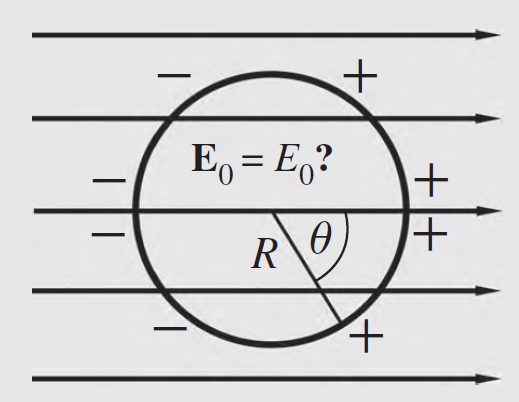
\includegraphics{2020/01/zangwill_fig_5_2.png}
    \caption{Zangwill Fig.~5.2.}
    \label{fig:zangwill_fig_5_2}
\end{figure}

Suppose now we have some strangely-shaped conductor with a cavity machined out of it, and we place a small (say, positive) charge inside the cavity. Well, what happens to the charge in the conductor? Clearly the inside surface of the cavity must rearrange itself to cancel the field within the conductor. That takes some net negative charge on the inside surface. That is, negative charge accumulates to shield the interior. That charge had to come from somewhere, though. There must be a net positive charge on the exterior surface which rearranges itself in some energetically favorable way. The neat thing is that the solution on the exterior surface doesn't depend at all on the shape of the cavity, or where the charge is placed inside. This is what we mean by shielding. Our conductor hides the details of the interior and reveals only the net charge contained within.
    
%week 3
% Tuesday lecture swapped with Friday section due to MLK day
\section{Thursday, January 23, 2020}
    In full generality, we have an expression for the electrostatic potential near some charge distribution $\rho(\vec r)$:
\begin{equation}
    \varphi(\vec r)  =\frac{1}{4\pi \epsilon_0} \int d^3 r' \frac{\rho(\vec r')}{|\vec r- \vec r'|}.
\end{equation}
However, this denominator is complicated; it depends both on $\vec r'$, which we integrate over, and also $\vec r$, which we don't. A very nice way to decompose this expression is in terms of Legendre polynomials, as
\begin{equation}
    \frac{1}{|\vec r - \vec r'|} = \sum_{l=0}^\infty \frac{r'{}^l}{r^{l+1}} P_l(\uv r \cdot \uv r').
\end{equation}
If We're only interested in the potential on e.g. the $z$-axis, then this might be a good expansion to use. In that case, integrating over $\uv r'$ is not too bad. But if we're interested in more general $\vec r$ (say, ranging over a sphere), we still want to separate the angles, and we can instead use the angle addition formula for the spherical harmonics, which says
\begin{equation}
    \frac{1}{|\vec r - \vec r'|} = \sum_{l=0}^\infty \frac{r'{}^l}{r^{l+1}} \frac{4\pi}{2l+1} \sum_{m=-l}^l Y_{lm}(\theta, \phi) Y_{lm}^*(\theta',\phi').
\end{equation}

\subsection*{Capacitance}
Recall that the capacitance is defined as
\begin{equation}
    C= \frac{Q}{V},
\end{equation}
where $V$ is the potential relative to infinity. In a sense, the self-capacitance is the capacitance of the object with the other plate being a hollow sphere of infinite radius.

We're going to skip the details of the capacitance matrix and many-conductor systems; our main interest will be in systems with precisely two conductors, i.e. capacitors. Typically we put a $+Q$ charge on one and a $-Q$ charge on the other. These charges produce a potential difference $V$ between the conductors, such that the ratio $C=Q/V$ is the capacitance.

The prototypical example is the parallel-plate capacitor, with two plates of area $A$ and charge $+Q$ and $-Q$. So long as the plate separation $d$ is much less than the lateral dimension $\sqrt{A}$, i.e. $\sqrt{A} \gg d$, we can approximate these as infinite plates. It follows that
\begin{equation}
    \vec E = - \frac{Q}{\epsilon_0 A} \uv z, \quad V = -\int_0^d E\, dz = \frac{Qd}{\epsilon_0 A},
\end{equation}
so that
\begin{equation}
    C= \frac{Q}{V} = \frac{\epsilon_0 A}{d}.
\end{equation}
Let's note that our plates aren't really infinite, so the fringing effects at the edges mean that the $E$-field is weaker at the edges. It follows that the potential difference is lower for the same charge, so the capacitance goes up. Apparently we have \emph{underestimated} the capacitance.

Now we can calculate the energy in the capacitor as
\begin{equation}
    U=\frac{1}{2}\int d^3 r \rho(\vec r) V(\vec r)
\end{equation}
Notice that if we have two conductors, this integral simplifies considerably. Suppose we have one conductor with a surface $S_1$ and a charge $+Q$ and another conductor with a surface $S_2$ and a charge $-Q$. Conductors are equipotentials, and it follows that since all the charge lies on the surface, the integral becomes
\begin{equation}
    U= \frac{1}{2} \bkt{\int_{S_1} d^2 S \sigma_+(\vec r) V_+ + \int_{S_2} d^2S \sigma_-(\vec r) V_-} = \frac{1}{2} \bkt{V_+ Q + V_- (-Q)} = \frac{1}{2} QV,
\end{equation}
since $V=V_+ - V_-$ is the difference in the potentials. We can rewrite this as
\begin{equation}
    U= \frac{1}{2} \frac{Q^2}{C} = \frac{1}{2} CV^2,
\end{equation}
and this has interesting consequences depending on whether we hold charge constant or voltage constant. That is, if we hold charge constant, then it makes sense that a higher-capacitance (in the case of parallel plates, smaller $d$) setup is energetically favored. But if we hold voltage constant, then the plates actually want to push apart (lower capacitance).

For our parallel plate capacitor, we can check that this works by integrating the energy in the $E$-field:
\begin{equation}
    U_\parallel = \frac{1}{2} \epsilon_0 \int E^2 d^3r = \frac{\epsilon_0}{2} \frac{Q^2}{\epsilon_0^2 A^2} Ad = \frac{1}{2} QV.
\end{equation}

\begin{exm}[The quantum dot]
    We've just found that the self-energy of an object is given by
    \begin{equation}
        U= \frac{Q^2}{2C}.
    \end{equation}
    For objects with large self-capacitances, adding a bit of charge doesn't affect the total energy much. But for very small objects on the nanoscale, this self-capacitance can be very small, so it may take a lot of energy to change the charge by a little bit. That is, $U$ looks like a parabola centered at zero, and if we apply a ``gate voltage,'' we can shift the zero over to e.g. $Q=1/2$, so that whether we have $0$ or $1$ (electron) charges in the dot, both are equally favorable from an energy standpoint. Adding temperature into the picture can mess this up, though. Once the energy scale $k_BT$ becomes comparable to the energy cost of adding a charge, thermal effects will destroy this nice zero-or-one picture.
\end{exm}
%things will get worse before they get better

\subsection*{Dielectrics (Zangwill Ch. 6)}
Conductors are nice because their charge carriers redistribute to cancel applied electric fields. But insulators are more complicated because their cancellation is imperfect due to subtle material properties.

In materials, we can write the total charge $\rho$ as a sum of two terms-- a free (applied) charge and a polarization/bound charge due to the material response. That is,
\begin{equation}
    \rho(\vec r) = \rho_f(\vec r) + \rho_P(\vec r).
\end{equation}
The free charge $\rho_f$ is charge we control by putting it on objects, while the polarization (bound) charge $\rho_P$ is how the material responds to the applied charge/fields. For instance, in conductors, all the $\rho_P$ (i.e. the induced charge) lies on the surface of the conductor.

If we consider a dielectric with no net charge, then
\begin{equation}\label{eqn:unchargeddielectric}
    \int_V d^3 r\, \rho_P(\vec r) + \int_S d^2S \, \sigma_P(\vec r) =0.
\end{equation}
That is, the sum of the polarization volume charge and the polarization surface charge is zero.

We can then motivate the polarization vector $\vec P(\vec r)$ in the following way. A polarization vector should describe how charges redistribute in a material, such that
\begin{gather}
    \vec P(\vec r) = 0 \text{ outside the material},\\
    \vec P(\vec r) \cdot \uv n = \sigma_P(\vec r) \text{ on surface}.
\end{gather}
We can plug this into our equation~\eqref{eqn:unchargeddielectric} to get
\begin{equation}
    \int_V d^3 r\, \rho_P(\vec r) + \int_V d^3r\, \div \vec P(\vec r) =0
\end{equation}
by the divergence theorem. Since these are both volume integrals, it follows that the integrand vanishes,
\begin{equation}\label{eqn:divp}
    \div \vec P(\vec r) = -\rho_P(\vec r) \text{ inside material.}
\end{equation}

We can now integrate the polarization over the volume of the material. Note that $\grad_i r_j= \delta_{ij}$, so
\begin{equation}
    \int_V d^3 r\, P_j  = \int d^3r\, P_i \grad_i r_j = \int_V d^3r\, \grad_i(r_j P_i) - \int_V d^3r \, r_j \grad_i P_i
\end{equation}
by the chain rule. Then the first term is a divergence, so we can turn it into a surface integral, i.e.
\begin{equation}
    \int_V d^3r\, P_j = \int_S d^2 S\, r_j \sigma_P(\vec r) + \int_V d^3 r \, r_j \rho_P(\vec r)
\end{equation}
using the definitions of the polarization volume charge and surface charge. But now we recognize that these are moment integrals of charge distributions, which means that these are precisely in the form of a dipole moment. That is,
\begin{equation}
    \int_V d^3r \,\vec P = \vec p,
\end{equation}
the net dipole moment of the distribution. Hence we can think of polarization as dipole moment per unit volume.

Question: which quantity has more information, $\vec P(\vec r)$ or $\rho(\vec r)$? A priori, we might think that because of Eqn.~\eqref{eqn:divp}, the charge density has less information than the polarization vector, since we've taken a derivative (which is a lossy operation). But if we take the integral $\int_V d^3r \vec P = \vec p$, we only specify one moment of the distribution.

As it turns out, the polarization has more information because it contains phase information. That is, the integral tells us one piece of information we can extract from $\vec P$, but there's in principle more we can do with $\vec P$.
\section{Friday, January 24, 2020}
    \begin{quote}
    \textit{``When I was in kindergarten... you know, it's like that Opus Dei thing. You punish yourself to see how much you can take.''}
    
    ---Nemanja Kaloper
\end{quote}

Let's conclude our proof of the Fourier theorem. We wrote the partial sum
\begin{equation}
    f_N(x) = \frac{1}{2\pi} \int_{-\pi}^\pi dt f(x+t) \frac{\sin\bkt{(N+1/2)t}}{\sin(t/2)},
\end{equation}
and said that due to the $2\pi$-periodicity, we could simply shift the domain of integration in $t$ as we like. If there's a single discontinuity at $x$, we can break up the domain of integration as
\begin{equation}
    \frac{1}{2\pi} \bkt{\int_{-\pi}^0 dt\,f(x+t) \frac{\sin\bkt{(N+1/2)t}}{\sin(t/2)}
    +\int_{0}^\pi dt\, f(x+t) \frac{\sin\bkt{(N+1/2)t}}{\sin(t/2)}}.
\end{equation}
Consider just the first term, the integral from $-\pi$ to $0$. We can add and subtract the function's limit from the left,
\begin{equation}
    f_N^- = \frac{1}{2\pi} \int_{-\pi}^0 \bkt{f(x^-) +\paren{f(x+t)-f(x^-)}} \frac{\sin \bkt{(N+1/2)t}}{\sin(t/2)}.
\end{equation}
We've just added zero. Hence the following integral can be evaluated as
\begin{equation}
    \frac{1}{2\pi} \int_{-\pi}^0 \bkt{f(x^-)} \frac{\sin \bkt{(N+1/2)t}}{\sin(t/2)} =\frac{f(x^-)}{2\pi} (\pi) = \frac{f(x^-)}{2}.
\end{equation}
We did the integral of the ratio of sines previously. On the interval $-\pi$ to $\pi$ it was $2$, and by the evenness of the ratio of sines, the integral over the half-interval $-\pi$ to $0$ is just $\pi$. 

Computing the integral $f_N^+$from $0$ to $\pi$, we get something very similar---the right limit of the function, $f(x^+)/2$, and another integral.
%When I was in kindergarten... you know, it's like that Opus Dei thing. You punish yourself to see how much you can take.

We shall argue that the integrals cancel each other perfectly by the Riemann-Lebesgue lemma, which (roughly) states that the integral of fast functions which oscillate a lot about a point are zero except about some region where the oscillations are slow.

That is, we wish to compute
\begin{equation}
    \frac{1}{2} \int_{-\pi}^0 dt \frac{f(x+t)-f(x^-)}{\sin(t/2)} \sin\bkt{(N+1/2) t}.
\end{equation}
Notice that for $t\to 0$ from the left, the numerator goes as $f(x^-)t$ since $f$ is continuous up to $x$. The denominator $\sin(t/2)$ is a slow function; it is $4\pi$ periodic and only goes to zero at $t\to 0$, where its leading order behavior is $\sin(t/2) \sim t/2$. In the limit as $N$ grows very large, we need only worry about the integrand near $t\to 0$. That is, it goes as $\sin((N+1/2)t) \sim (N+1/2) t + O(t^3)$. Hence our slow function is approximately
\begin{equation}
    \sigma(t) = \frac{f(x+t)-f(x^-)}{\sin(t/2)} \approx \frac{f'(x^-)t}{t/2} = 2f'(x^-),
\end{equation}
%if you can't explain your idea without equations then you don't know what is going on.
so that
\begin{equation}
    \lim_{N\to \infty} \int_a^b dt \, \sigma(t) \sin((N+1/2) t) = 0.
\end{equation}
That is, this integral oscillates so fast and our slow function is well-behaved on the whole integral, so the whole integral vanishes. This is the conclusion of the Riemann-Lebesgue lemma.

Let's do a trick to see this works. Let $\omega = N+1/2$, and define a new variable
\begin{equation}
    t = t'  + \frac{\pi}{N+1/2} = t' + \frac{\pi}{\omega}
\end{equation}
so that
\begin{equation}
    \int_{a-\pi/\omega}^{b-\pi/\omega} dt' \, \sigma(t' + \pi/\omega) \sin(\omega (t' +\pi/\omega)) = -\int_{a-\pi/\omega}^{b-\pi/\omega} dt' \, \sigma(t' + \pi/\omega) \sin(\omega t')
\end{equation}
since the $\sin$ is $2\pi$-periodic. This is clearly the same as our original integral, since we've just changed variables. Call the integral $I$. Then
\begin{equation}
    2I = \int_a^b dt \, \sigma(t) \sin(\omega t) - \int_{a-\pi/\omega}^{b-\pi/\omega} dt\, \sigma(t + \pi/\omega) \sin (\omega t).
\end{equation}
We see that as $\omega \to \infty$, these integrals perfectly cancel each other. More precisely, we get an integral
\begin{equation}
    \int_a^{b-\pi/\omega} dt \sin(\omega t) \bkt{\sigma(t) - \sigma(t+\pi/\omega)}-\int_{a-\pi/\omega}^a dt \, \sigma (t + \pi/\omega) \sin \omega t + \int_{b-\pi/\omega}^b dt \sigma(t) \sin \omega t.
\end{equation}
If we take the last two terms, we see they are both bounded. The last two are bounded by some multiple of $\pi/\omega$, since the interval from $b-\pi/\omega$ to $b$ becomes infinitesimal and the functions $\sigma(t), \sin(\omega t)$ are well-behaved around $b$. A similar argument applies for the integral from $a-\pi/\omega$ to $a$.
%If you want to live a stable steady life, don't live too dangerously. Stay away from fast guys.

The first term is also bounded and vanishes since $\sigma(t) -\sigma(t+\pi/\omega)$ is just a derivative $\sigma'(t)$ times $\pi/\omega$, and $\sigma'$ is well-behaved (nonsingular) over the interval. It follows that in the limit as $\omega \to \infty$, all these integrals go to zero, so that indeed $I=0$ and
\begin{equation}
    \lim_{N\to \infty} f_N(x) = \frac{f(x^-) + f(x^+)}{2},
\end{equation}
and moreover we recover the completeness relation
\begin{equation}
    \lim_{N\to \infty} \frac{\sin(N+1/2)(x-t)}{\sin(\frac{x-t}{2})} = \delta(x-t).
\end{equation}

\subsection*{Complex analysis}
A complex number is a pair $(x,y)$, which we may write
\begin{equation}
    z = x+iy, \quad x,y\in \RR
\end{equation}
in cartesian form. Complex numbers also have a polar form,
\begin{equation}
    z = \rho e^{i\phi}, \quad \tan \phi =y/x, \quad \rho = \sqrt{x^2+y^2}.
\end{equation}

Complex functions on the complex plane may be multivalued. For instance, consider the function $\ln z$. If we write a number like $A = Ae^{2\pi n i}$, $n\in\ZZ$, then
\begin{equation}
    \log A = \log (Ae^{2\pi n i}) = \log A + 2\pi n i,
\end{equation}
so the log is infinitely multivalued. We consider complex functions
\begin{equation}
    f: \CC \to \CC,
\end{equation}
mapping some $z \in \CC$ to $w\in \CC$, and since the output is complex, we can write
\begin{equation}
    f(z) = u(x,y) + i v(x,y)
\end{equation}
where now $u,v: \CC \to \RR$ are real-valued functions. Arbitrary complex functions are clearly as complicated as real functions, but there is a special subset of complex functions which are more constrained in interesting ways. These are the \emph{analytic functions.}
    
%week 4
\section{Tuesday, January 28, 2020}
    Last time, we discussed the field from a charge at the boundary between two dielectrics. At the boundary, $E_\perp$ is discontinuous because of the surface charge. But $\vec D$ seems to be continuous since it depends only on the free charge. What's happening? Why does $E$ have a curl if $D$ is continuous? Really, what's happening is that $D$ also knows about the polarization:
\begin{equation}
    \curl \vec D = \curl \vec P.
\end{equation}
So $E$ can be composed of a curl part and a divergence part, and the polarization itself is sourcing a curl at the boundary.

\subsection*{Poisson and Laplace equations}
%``Everyone uses their own words, especially Professor Kaloper.''
Let us leave behind the world of matter for a bit and explore Laplace's equation. To begin our discussion, suppose we have two solutions of Poisson's equation,
\begin{equation}
    \nabla^2 \varphi_1 + \nabla^2 \varphi_2 = -\frac{\rho(\vec r)}{\epsilon}.
\end{equation}
When are solutions unique? Define
\begin{equation}
    \Phi = \varphi_1 - \varphi_2.
\end{equation}
By linearity, it follows that
\begin{equation}
    \nabla^2 \Phi = 0.
\end{equation}
In general, note that for scalar functions $f,g$, we have
\begin{equation}
    \int_S d\vec S \cdot f\grad g = \int_V d^3r \, \div(f\grad g) =\int_V d^3r (f\nabla^2 g + \grad f \cdot \grad g).
\end{equation}
If we take $f=g=\Phi$, then
\begin{equation}
    \int_S d\vec S \cdot \Phi \grad \Phi = \int_V d^3 r \paren{\Phi \underbrace{\nabla^2 \Phi}_\text{=0} + |\grad \Phi|^2} \geq 0.
\end{equation}
This first term is zero by assumption, while the second term is positive semi-definite and equal to zero only for $\grad \Phi=0$.

When does the LHS vanish? Either $\Phi$ vanishes on the boundary or $\grad \Phi\cdot \uv n$ vanishes on the boundary, i.e. the normal derivative is zero. Either way, we get $\grad \Phi=0$, which forces $\Phi={}$constant.

If $\Phi=0$ on $S$, then these are the Dirichlet boundary conditions, and in fact $\varphi_1 = \varphi_2=$some known values on $S$. Alternately, if $\uv n \cdot \grad \Phi=0$, then that's equivalent to specifying the normal derivative $\uv n \cdot \grad \varphi$ on the boundary. These are \term{Neumann boundary conditions}, and the solutions can vary by a constant. We could also specify the value on part of the boundary and a normal derivative elsewhere; these are mixed or Cauchy boundary conditions.

This tells us when solutions are unique, though it does not prove existence. In general we need only specify $\varphi$ or $\uv n\cdot \grad \varphi$ on the boundary; if we try to fix both, the problem will usually be overdetermined unless we're very lucky.

Let us make a guess when we try to solve Laplace's equation. We will make the following ansatz:
\begin{equation}
    \varphi(u,v,w) = A(u) B(v) C(w)
\end{equation}
in terms of some functions $A,B,C$. If we make this guess and plug it into the differential equation, then our PDE separates into ODEs for each variable, linked by separation constants. While this seems like a really simple guess, Zangwill says that this works in 13 different coordinate systems.%
    \footnote{I haven't checked.}

Zangwill also claims to write down the general solution to Laplace's equation, but it's not true. \emph{Do not believe Zangwill Eqn. 7.14.} When the equation separates, we get two linearly independent solutions for $A$, two for $B$, and two for $C$ (the equation is second-order). That is, we have
\begin{equation}
    A, \Tilde{A}; B,\Tilde{B}; C, \Tilde{C}.
\end{equation}
In fact, each ODE might give us a family of eigenfunctions (think of sines in a rectangular waveguide) indexed by some eigenvalues. So we really have
\begin{equation}
    \set{A_\alpha, \Tilde{A}_\alpha}; \set{B_\beta,\Tilde{B}_\beta}; \set{C_\gamma, \Tilde{C}_\gamma},
\end{equation}
and to construct the most general solution, we need $8$ terms:
\begin{equation}
    \varphi=\sum_{\alpha,\beta,\gamma} \bkt{a^{(1)}_{\alpha \beta \gamma} A_\alpha(u) B_\beta(v) C_\gamma(w) + a^{(2)}_{\alpha \beta \gamma} A_\alpha(u) B_\beta(v) \tilde C_\gamma(w) + a^{(3)}_{\alpha \beta \gamma} A_\alpha(u) \tilde B_\beta(v) C_\gamma(w) + \dots}.
\end{equation}
This is precisely equivalent to the construction of entangled states in quantum mechanics. That is, the most general solution isn't just a product of individual solutions but a sum of products. It is a tensor product structure, not a direct product. Contrast Zangwill 7.14, which claims the most general solution is
\begin{equation}
    \sum_{\alpha \beta \gamma}(a_\alpha A_\alpha(u) + \tilde a_\alpha \tilde A_\alpha(u)) (b_\beta B_\beta (v) + \tilde b_\beta \tilde B_\beta(V) ) (c_\gamma C_\gamma(w) + \tilde c_\gamma \tilde C_\gamma(w)).
\end{equation}
This is just a product of solutions, but there aren't enough parameters for the solution space. There are really only four independent parameters here, since we can pull out an $a_\alpha b_\beta c_\gamma$ and treat this as a single number.

Now, in the theory of Sturm-Liouville problems, ODEs satisfying self-adjointness provide us with a complete orthonormal set of eigenfunctions. Completeness says that
\begin{equation}
    \sum_k \psi_k(v) \psi_k^*(v') = \delta(v-v'),
\end{equation}
where $k$ indexes over eigenfunctions. It follows that we have a basis, so that
\begin{equation}
    F(v) = \int \delta(v-v') F(v') dv' = \sum_k \underbrace{\int dv' \psi_k^*(v') F(v')}_{F_k} \psi_k(v) = \sum_k F_k \psi_k(v).
\end{equation}
That is, we can decompose $F(v)$ into its components. Note that if $F(v) = \psi_k'(v)$, then we immediately have $F_k =\int dv' \psi_k^*(v') \psi_{k'}(v') =\delta_{kk'}$.

In Cartesian coordinates, separation of variables is very nice. We have
\begin{equation}
    \nabla^2 \varphi = 0, \quad \varphi(x,y,z) = X(x) Y(y) Z(z).
\end{equation}
If we plug in and divide by the original function $\varphi$, we get
\begin{equation}
    -\frac{X''}{X} = \frac{Y''}{Y} + \frac{Z''}{Z}.
\end{equation}
Since the LHS depends only on $x$ and the RHS depends only on $Y$ and $Z$, we can write
\begin{equation}
    X'' = \alpha^2 X \implies X(x) = \begin{cases}
        A_0 + B_0 x & \alpha = 0\\
        A_\alpha e^{\alpha x}  + B_\alpha e^{-\alpha x} & \alpha \neq 0.
    \end{cases}
\end{equation}
As we expected, there are two linearly independent solutions ($1$ and $x$ for $\alpha=0$ and $e^{\pm x}$ for $\alpha \neq 0$.

For instance, we could set up a box (say, a cube of side length $a$) where the boundary condition is $V_1(x,y)$ at $z=0$ and $V=0$ on the sides. It follows that the $X$ and $Y$ dependence is sines which are periodic in $a$, namely
\begin{equation}
    V(x,y,z) = \sum_{m=1}^\infty \sum_{n=1}^\infty V_\text{mn} \sin \frac{m\pi x}{a} \sin \frac{n\pi y}{a} \frac{\sinh \gamma_{mn}(a-z)}{\sinh \gamma_{mn}a},
\end{equation}
such that
\begin{equation}
    \gamma_{mn}^2 = \paren{\frac{m\pi}{a}}^2 + \paren{\frac{n\pi}{a}}^2.
\end{equation}
This now satisfies $V(z=a)=0$, and the coefficients $V_{mn}$ are given by taking the Fourier components of the boundary condition $V_1(x,y)$, i.e.
\begin{equation}
    V_{mn}^{(1)} = \frac{4}{a^2} \int_0^a dx \int_0^a dy \, V_1(x,y) \sin \frac{m\pi x }{a} \sin \frac{n\pi x}{a}.
\end{equation}
What if another wall had a nontrivial boundary condition, e.g. $V_2(y,z)$ at $x=a$? Fortunately, Poisson's equation is linear and homogeneous so we can just add solutions. That is, we can add on a solution
\begin{equation}
    V_2(x,t,z) = \sum_{m=1}^\infty \sum_{n=1}^\infty V^{(2)}_\text{mn} \sin \frac{m\pi y}{a} \sin \frac{n\pi z}{a} \frac{\sinh \gamma_{mn}(x)}{\sinh \gamma_{mn}a}.
\end{equation}

\begin{exm}
    Let's consider the solution to Laplace's equation in a Faraday cage. Suppose we have two rows of infinite wires. The wires are separated within the rows by a distance $a$ and the two rows are separated by a distance $d$ (so one is at $z=0$ and one is at $z=d$). Say the row extends in the $x$ direction and the wires extend in the $y$ direction. Each wire has linear charge density $\lambda$.
    
    The charge density from the lower row of wires is
    \begin{equation}
        \sigma(x) = \lambda \sum_{p=-\infty}^\infty \delta(x-pa).
    \end{equation}
    Because the charge distribution is symmetric (even) about the origin, we can write our charge distribution in terms of cosines,
    \begin{equation}
        \sigma(x) = A_0 + \sum_{m=1}^\infty A_m \cos \frac{2\pi m x}{a}.
    \end{equation}
    This will turn out to be Neumann boundary conditions, since we're specifying a charge distribution on the boundary, which fixes the perpendicular component of the $E$-field at the boundary and therefore the normal derivative of $V$.
    
    The coefficients are given by
    \begin{equation}
        A_0 = \frac{1}{a} \int_{-a/2}^{a/2} dx\, \sigma(x)  = \frac{\lambda}{a}, \quad A_m =\frac{2}{a} \int_{-a/2}^{a/2} dx \,\sigma(x) \cos \frac{2\pi mx}{a} = \frac{2\lambda}{a}.
    \end{equation}
    Since our period is $a$, we only ever see the delta function at the origin. We    Since our charge density has a period $a$, we only ever see the delta function at the origin. We'll continue this next time.
\end{exm}
\section{Thursday, January 30, 2020}
    Let's finish our discussion from last time of the Faraday cage. The Fourier decomposition of the charge distribution is
\begin{equation}
    \sigma(x,z=0) = \frac{\lambda}{a} + \sum_{m=1}^\infty \frac{2\lambda}{a} \cos \frac{2\pi mx}{a},\label{eq:faradaychargedensity}
\end{equation}
and we see that cosines in $x$ are part of the separable solutions to Laplace's equation in Cartesian coordinates. The wires extend in the $y$ direction, so we want a constant solution in $y$, and it just remains to fit the $z$-dependence.

Note that $\sigma$ specifies a normal derivative of $\varphi$ (it is a discontinuity in $E$), so our general solution could look like
\begin{equation}
    \varphi(x,y,z) = (ax+ b|z| +cx|z| + d) + \sum_\gamma c_\gamma \cos(\gamma x) e^{-\gamma|z|}.
\end{equation}
But by the symmetry in $x$, the terms linear in $x$ go away and the constant $d$ can be set to zero WLOG. There's no $e^{+\gamma|z|}$ terms since this would diverge as $|z|\to \infty$. Thus we're left with
\begin{equation}
    \varphi(x,y,z) = b|z| + \sum_\gamma c_\gamma \cos(\gamma x) e^{-\gamma|z|}.
\end{equation}
If we now take the normal derivative at $z\to 0$, we get
\begin{equation}
    \P{\varphi}{z}|_{z\to 0^+} =b+ \sum_\gamma c_\gamma(\cos(\gamma x)) (-\gamma) e^{-\gamma(0)}
\end{equation}
and 
\begin{equation}
    \P{\varphi}{z}|_{z\to 0^-} =-b+ \sum_\gamma c_\gamma(\cos(\gamma x)) (\gamma) e^{\gamma(0)}.
\end{equation}
It follows that the electric fields are
\begin{gather}
    E_\perp(z\to 0^+) = -\P{\varphi}{z}|_{z\to 0^+} = - b+  \sum_\gamma c_\gamma(\cos(\gamma x)) \gamma,\\
    E_\perp(z\to 0^-) = -\P{\varphi}{z}|_{z\to 0^-} = +b - \sum_\gamma c_\gamma(\cos(\gamma x)) \gamma.
\end{gather}
If we now take their difference, we have
\begin{equation}
    \frac{\sigma}{\epsilon_0} = E_\perp(z\to 0^+) - E_\perp(z\to 0^-) = -2b + 2 \sum_\gamma c_\gamma(\cos\gamma x) \gamma.
\end{equation}
By matching coefficients with Eq.~\eqref{eq:faradaychargedensity}, we find that
\begin{equation}
    -2b=\frac{\lambda}{\epsilon_0 a}, \quad \gamma = \frac{2\pi}{a}m, \quad c_\gamma = \frac{\lambda}{a\gamma \epsilon_0}= \frac{\lambda}{\epsilon_0 2\pi m}
\end{equation}
Plugging back into our solution, we have
\begin{equation}
    \boxed{\varphi(x,y,z) = -\frac{\lambda}{2a \epsilon_0} |z| + \frac{\lambda}{2\pi \epsilon_0} \sum_{m=1}^\infty \frac{1}{m} \cos \frac{2\pi m}{a} e^{-\frac{2\pi m}{a} |z|}.}
\end{equation}
This diverges far away due to the $|z|$ term, but that actually makes sense because far from the cage (at large $z$, we see the field of an infinite plane of charge, i.e. a constant field and a potential changing linearly with distance.

That's the solution for a single wire plane. If we add two such planes separated by a distance $d$, then we have
\begin{equation}
    \varphi(x,y,z) = -\frac{\lambda}{2a\epsilon)} \overbrace{\paren{|z| + |d-z|}}^{{}=d\text{ ``inside,'' }0 < z < d} + \sum \dots
\end{equation}
and the exponential terms both decay inside exponentially fast.

We can discuss separable solutions to Laplace's equation in some generality. For Cartesian coordinates, there are three separation constants $\alpha,\beta,\gamma$ with $\alpha^2 + \beta^2 + \gamma^2 =0$, It follows that most of our solutions will have oscillation in at least one direction and decay (or growth) in another. For spherical solutions, there are technically two independent solutions for the $\theta$ dependence, the associated Legendre polynomials $P_l^m$ and the other kind $Q_l^m$. The second kind are divergent at $\theta=\pi$ and sometimes at $\theta=0$. Cylindrical solutions have many different options; the radial dependence can be growing exponentially, decaying exponentially, growing as a log, or oscillating/decaying as cylindrical Bessel functions. We won't really discuss this in any large degree of detail, but it's good to be aware that such solutions exist.%
    \footnote{Arfken has a very detailed discussion of Bessel functions and Legendre polynomials}

\begin{exm}
    Consider a ring of charge $Q$ and radius $R$. If we consider this in a spherical expansion, we can write
    \begin{equation}
        \varphi(r,\theta,\phi) = \begin{cases}
            \sum_{l=0}^\infty \frac{B_l}{r^{l+1}} P_l(\cos\theta) & r > R,\\
            \sum_{l=0}^\infty A_l r^l P_l(\cos\theta)& r< R.
        \end{cases}
    \end{equation}
    But since these solutions must agree at $r=R$, we can actually write
    \begin{equation}
        \varphi(r,\theta,\phi) = \begin{cases}
            \sum_{l=0}^\infty c_l \frac{R^{l+1}}{r^{l+1}} P_l(\cos\theta) & r > R,\\
            \sum_{l=0}^\infty c_l \frac{r^l}{R^l} P_l(\cos\theta)& r< R.
        \end{cases}
    \end{equation}
    Moreover, we can explicitly calculate
    \begin{equation}
        \varphi(r,0,0) = \frac{1}{4\pi \epsilon_0 } \frac{Q}{\sqrt{r^2+R^2}} = \frac{Q}{4\pi \epsilon_0 R} \sum_{l=0}^\infty \paren{\frac{r}{R}}^l P_l(0)
    \end{equation}
    for $r<R$ and the expansion of $\frac{1}{\sqrt{1-2tz + t^2}}$. Now we can just evaluate our general expansion for $r<R$ at $\theta=\pi/2$ using the fact that $P_l(\cos(\theta=\pi/2))=1$. Matching the $r$ dependence, we find that
    \begin{equation}
        c_l = \frac{Q}{4\pi \epsilon_0 R} P_l(0).
    \end{equation}
    It's a bit like analytic continuation---if we know a function on some line, we can actually extend it consistently elsewhere. Now that we have the coefficients $c_l$, we have the solution for $\varphi$.
\end{exm}

\begin{exm}
    Consider a solid grounded conductor with a ``bite'' taken out of it. Suppose we can analyze this system in cylindrical coordinates with translational symmetry along the $z$-axis. Then our solution (in almost full generality: see our discussion from last time) is
    \begin{equation}
        \varphi(\rho,\phi,z) = (A_0+ B_0 \ln \rho)(C_0 \phi + D_0) + \sum_{\alpha \neq 0} \bkt{A_\alpha \rho^\alpha _\alpha \rho^{-\alpha}} \bkt{C_\alpha e^{i\alpha \phi} + D_\alpha e^{-i\alpha \phi}}.
    \end{equation}
    This will be the general solution so long as one of $A_\alpha,B_\alpha,C_\alpha,D_\alpha$ is zero for each $\alpha$. We'd like to avoid singularities as $\rho \to 0$. We can now write
    \begin{equation}
        \varphi(\rho\to 0,\phi,z) \propto \rho^{\pi/\beta} \sin\frac{\pi \phi}{\beta}
    \end{equation}
    as the leading dependence. That is, we've thrown away the $\rho^{-\alpha}$ and $\ln \rho$ dependence, and we also got rid of $C_0$ in order for our potential to be single-valued.
    
    If we look at $\vec E = -\grad \varphi$, we notice that
    \begin{equation}
        \P{\varphi}{\rho} \propto \frac{\pi}{\beta} \rho^{\pi/\beta - 1} \sin \frac{\pi \phi}{\beta},
    \end{equation}
    and we can now see that if $\beta > \pi$ (i.e. we have a spike, not a bite) then the corner will have very large electric fields at small $\rho$.
\end{exm}

\begin{exm}
    Finally, let us consider two cylindrical rods aligned along the $z$-axis, separated by a little gap. We hold the rod at positive $z$ at a potential $V_R$ and the rod at negativ $z$ at a potential $V_L$. What is the potential inside the gap? There is no $\phi$ dependence, so $\alpha=0$ (we don't get the power-law decay/growth in $\rho$). Our boundary conditions are given in $\phi,z$, so we will take the separation constant $k^2<0$ to expand in $z$, and define $k=i\kappa$ as is conventional.
    
    This means we're expanding in Bessel functions $I$ and $K$, and since $K$ diverges as $\rho \to 0$, we will be using the functions $I$. THus
    \begin{align}
        \varphi(\rho,\phi,z) &= \frac{1}{2\pi} \int_0^\infty I_0(\kappa \rho) (E(\kappa) e^{i\kappa z} + F(\kappa) e^{-i\kappa z}) d\kappa + \text{constant}\
            &= \frac{1}{2\pi} \Int A(\kappa) I_0(|\kappa|\rho) e^{i\kappa z} d\kappa + \text{constant.}
    \end{align}
    That is, we extended the limits of integration to $-\infty,\infty$ and now we recognize this integral as a Fourier transform. We can recover $A(\kappa) I_0(|\kappa|\rho)$ by taking an inverse Fourier transform.
\end{exm}

%week 5
\section{Tuesday, February 4, 2020}
    Midterm logistics---we'll have the midterm Friday, during the regular section time. There will be 3-4 questions, of which we will choose a few and solve them in class. The full exam will then become a take-home which we'll work on over the weekend. Content runs through the Laplace chapter and not the Poisson chapter. In-class and take-home portions will be equally weighted (50/50).

\subsection*{Poisson's equation}
Laplace's equation is a special case of Poisson's equation. That is, Poisson's equation reads
\begin{equation}
    \nabla^2 \varphi = -\frac{\rho}{\epsilon_0}
\end{equation}
for vacuum or electric fields in (not-dielectric) matter, while
\begin{equation}
    \nabla^2 \varphi = -\frac{\rho_f}{\epsilon}
\end{equation}
in matter, where $\epsilon$ is the permittivity. This latter form is sometimes nice when we know the free charge.

A useful technique for solving boundary value problems in electrostatics is the \term{method of images}. We'll start with the classic example, a charge above a grounded plane.

\begin{exm}
    Suppose we have some charge $q$ a distance $z_0>0$ above a grounded conducting plane, $\varphi=0$. The method of images says that we can solve potential boundary value problems by matching the potential with an equivalent fictitious charge distribution.
    
    Notice that we can produce this same potential in the $z>0$ half-space if we place an ``image charge'' at $-z_0$. The potential from this distribution is
    \begin{equation}
        \varphi(x,y,z) = \frac{q}{4\pi \epsilon_0} \bkt{\frac{1}{\sqrt{x^2+y^2+(z-z_0)^2}} - \frac{1}{\sqrt{x^2+y^2+(z+z_0)^2}}}.
    \end{equation}
    The first term is the Poisson solution corresponding to our real charge, while the second term solves Poisson's equation in the upper half-space, so this will overall satisfy Poisson's equation for the \emph{real} charge distribution in the space we care about.
    
    One can easily check that on the plane $z=0$, we have $\varphi(x,y,0) =0$, so the boundary condition is satisfied.
    
    Notice that the potential from the plane below it ($z<0$) is its potential above, up to a $z\to -z$. That is,
    \begin{equation}
        \varphi_\text{plane} (x,y,z<0) = -\frac{q}{4\pi \epsilon_0 \sqrt{x^2+y^2 + (-z+z_0)^2}}.
    \end{equation}
    But that tells us that
    \begin{equation}
        \varphi_\text{plane} + \varphi_\text{charge} = 0 \text{ for } z<0,
    \end{equation}
    which we expected. The conductor has screened out the influence of the charge in the lower half-space.
    
    We can calculate the energy of this configuration by taking%
        \footnote{I did this a little differently from lecture. This is the field of two point charges separated by a distance $2z$.}
    \begin{equation}
        q\int_{z_0}^\infty dz\, E(z) = \int_{z_0}^\infty dz \frac{q^2}{4\pi \epsilon_0 (2z)^2} = \frac{q^2}{4\pi \epsilon_0} \paren{-\frac{1}{4z_0}}.
    \end{equation}
    
    Equivalently this is half of the interaction energy of the charge and the image charge; we can see this by integrating over the energy in the field of two real charges and then arguing by symmetry that we only have field in the half-space, so the actual energy is half the energy of the real dipole.
    
    We can now calculate the charge distribution by looking at the normal derivative of potential at the conductor. Here,
    \begin{equation}
        -\P{\varphi}{z}|_{z=0^+} = \frac{\sigma}{\epsilon_0}.
    \end{equation}
    We have
    \begin{equation}
        \sigma/\epsilon_0 = \frac{q}{4\pi} \bkt{-\frac{z_0}{(\rho^2 + z_0^2)^{3/2}} - \frac{z_0}{(\rho^2+z_0^2)^{3/2}}},
    \end{equation}
    so then the total induced charge is
    \begin{align*}
        Q &= \int_0^\infty (2\pi \rho d\rho) \sigma(\rho,\phi)\\
            &= \int_0^\infty (2\pi \rho d\rho) \frac{q}{4\pi} \bkt{-\frac{z_0}{(\rho^2 + z_0^2)^{3/2}} - \frac{z_0}{(\rho^2+z_0^2)^{3/2}}}\\
            &= -q \int_0^\infty d\rho \frac{\rho z_0}{(\rho^2 +z_0^2)^{3/2}}\\
            &= \frac{q z_0}{(\rho^2+ z_0^2)^{1/2}}|_0^\infty\\
            &= -q.
    \end{align*}
    We learn that the induced charge was exactly equal and opposite to the real charge, as we might have guessed.
\end{exm}

\begin{exm}
    Let us now revisit a situation we've considered before. We have a charge $+q$ embedded in some dielectric of dielectric constant $\kappa_L$ which fills the region $z<0$, a distance $d$ from the interface with a different dielectric $\kappa_R$ which fills $z>0$.
    
    Emboldened by our success with the conducting plane, we might think that perhaps an image charge approach could work for the interface between dielectrics as well. That is, let's cook up a scenario where there's some image charge $q_R$ in a dielectric $\kappa_L$ on the right. It doesn't matter that the image charge configuration has $\kappa_L$ on the right now, since we just want to fit the boundary conditions at $z=0$.
    
    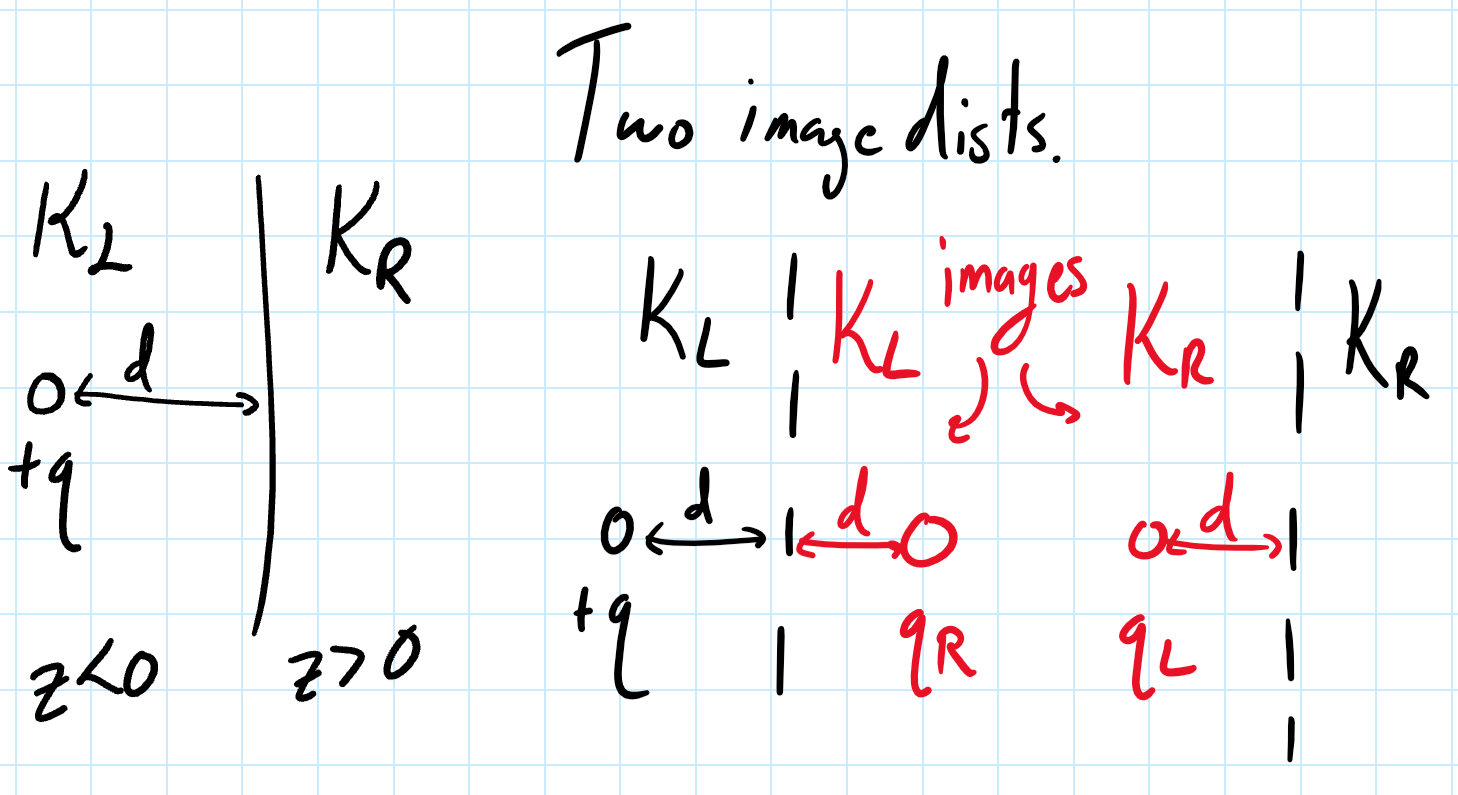
\includegraphics[width=0.95\textwidth]{2020/02/20200204_dielectric_images}
    
    It follows that the potentials in each region are
    \begin{gather}
        \varphi_L(x,y,z) = \frac{1}{4\pi \epsilon_L} \bkt{\frac{q}{\sqrt{x^2+y^2+(z+d)^2}} + \frac{q_R}{\sqrt{x^2+y^2+(z-d)^2}}},\\
        \varphi_R (x,y,z) = \frac{1}{4\pi\epsilon_R} \frac{q_L}{\sqrt{x^2+y^2+(z+d)^2}}.
    \end{gather}
    %
    The potential is continuous,
    \begin{equation}
        \varphi_L(x,y,0) = \varphi_R(x,y,0),
    \end{equation}
    while its normal derivative is discontinuous,
    \begin{equation}
        \kappa_L \epsilon_0 \P{\varphi_L}{z}|_z=0 = \kappa_R \P{\varphi_R}{z}|_{z=0}.
    \end{equation}
    Continuity tells us that
    \begin{equation}
        \frac{q+q_R}{\kappa_L} = \frac{q_L}{\kappa_R},
    \end{equation}
    and the normal derivative gives the condition that
    \begin{equation}
        -q d + q_R d = -q_L d.
    \end{equation}
    That is,
    \begin{equation}
        q=q_R + q_L.
    \end{equation}
    We now have two equations relating $q,q_R,$ and $q_L$, which we can easily solve
    \begin{equation}
        q_L = \frac{2\kappa_R}{\kappa_R + \kappa_L}q, \quad q_R = \frac{\kappa_L-\kappa_R}{\kappa_L + \kappa_R}q.
    \end{equation}
    We can then check that for $\kappa_L=\kappa_R$, we have $q_R=0$ and $q_L=q$. This says there's no image charge on the right (there's no boundary) and our left image charge is just the original charge.
\end{exm}

Like in Gauss's law, image charges only really work when we have a large amount of symmetry.
\section{Thursday, February 6, 2020}
    Today, we'll discuss Green's functions. The principle behind Green's functions is this. Consider an inhomogenous differential equation like the Poisson equation,
\begin{equation}
    \nabla^2 \varphi(\vec r) = -\frac{\rho(\vec r)}{\epsilon_0}.
\end{equation}
A Green's function is the inverse of the differential operator. It is the solution to the inhomogenous equation with a delta function source, i.e. for $\rho(\vec r) = \delta(\vec r - \vec r')$,
\begin{equation}\label{eqn:poissongreenfn}
    \nabla^2 G(\vec r, \vec r') = -\frac{1}{\epsilon_0} \delta(\vec r - \vec r').
\end{equation}
In fact, we know what potential corresponds to a point charge:
\begin{equation}
    G_0(\vec r, \vec r') = \frac{1}{4\pi \epsilon_0} \frac{1}{|\vec r - \vec r'|}.
\end{equation}
Strictly, Zangwill calls this the free-space Green's function because for any solution of Poisson's equation, we can simply add another solution of Laplace's equation (the homogeneous equation). In general the exact solution will have to be fixed by boundary conditions. Trivially, we can write that
\begin{equation}
    \int d^3 r' \, \rho(\vec r') \delta(\vec r-\vec r') = \rho(\vec r).
\end{equation}
If we multiply both sides of Eq.~\eqref{eqn:poissongreenfn} by $\rho(\vec r')$ and perform the $\vec r'$ integral, we get
\begin{equation}
    \nabla^2 \int d^3 r' \, G(\vec r,\vec r') \rho(\vec r') = -\frac{1}{\epsilon_0} \int d^3 r' \, \rho(\vec r') \delta(\vec r- \vec r') = -\frac{\rho(\vec r)}{\epsilon_0}.
\end{equation}
We conclude that in fact
\begin{equation}
    \varphi(\vec r) = \int d^3 r' \, G(\vec r, \vec r') \rho(\vec r').
\end{equation}
That is, the Green's function lets us build the solution to the inhomogeneous equation by integrating over (appropriately weighted) point charge potentials.

When we come to boundary value problems, there's an added complication. The potential of a point charge in a grounded box (and therefore its field) looks quite different than a potential in empty space. Let's start our discussion as follows:
\begin{equation}
    \int d\vec S' \cdot f\grad' g = \int d^3 r' \grad'\cdot (f\grad' g) = \int d^3 r' \bkt{\grad' f \cdot \grad' g + f \nabla'{}^2 g}.
\end{equation}
This is just a vector calculus manipulation. If we swap $f$ and $g$ and subtract from our original equation, we get
\begin{equation}
    \int d\vec S ' \cdot \bkt{f\grad' g - g \grad' f} = \int d^3 r' \bkt{f\nabla'{}^2 g - g\nabla'{}^2 f}.
\end{equation}
Let us now take
\begin{equation}
    f(\vec r') = \varphi(\vec r'), \quad g(\vec r') = G(\vec r, \vec r').
\end{equation}
Then
\begin{equation}
    \int d\vec S' \cdot \bkt{\varphi \grad' G - G \grad' \varphi} = \int d^3 r' \bkt{\varphi \grad'{}^2 G - G \grad'{}^2 \varphi} = -\frac{1}{\epsilon_0} \varphi(\vec r) + \frac{1}{\epsilon_0} \int d^3 r' G(\vec r, \vec r') \rho (\vec r').
\end{equation}
Hence we get back our inhomogenous solution, the $d^3r'$ integral, plus a homogenous solution given by the $d\vec S'$ integral. This surface term is very nice---if $\varphi$ is prescribed on the boundary (Dirichlet boundary conditions) then we can evaluate the first term in
\begin{equation}
    \int d\vec S' \cdot \bkt{\varphi \grad' G - G \grad' \varphi},
\end{equation}
and moreover if $G=0$ on the boundary then we just have to compute the first integral. Conversely if we had Neumann boundary conditions, then we should set $\uv n \cdot \grad' G =0$ so that the normal derivative of $G$ vanishes and we need only compute the second term.

\begin{exm}[``Splitting'']
    Let's consider Zangwill's third example. We wish to construct $G_D(\vec r, \vec r')$, the Green's function for a particular set of Dirichlet boundary conditions, $G_D(\vec r, \vec r')=0$ for $\vec r$ on some surface. We now remark that the Dirichlet Green's function can be written as a sum
    \begin{equation}
        G_D(\vec r, \vec r') = G_0 (\vec r, \vec r') + \Lambda(\vec r, \vec r') = \frac{1}{4\pi \epsilon_0} \frac{1}{|\vec r - \vec r'|} +\Lambda (\vec r, \vec r'),
    \end{equation}
    where $\Lambda$ solves the homogeneous equation (the Laplace equation).
    
    For instance, consider a point charge in a cylinder of length $L$ and radius $R$. The process of constructing the Green's function is as follows. Consider the potential sourced by the point charge in empty space. We can solve for the potential on the cylinder, and then solve Laplace's equation for some $\Lambda$ with \emph{minus} that potential as the boundary conditions. If we add the two solutions, we get the field of a point charge in a grounded cylinder which appears in our ordinary $\int d^3 r' G(\vec r, \vec r')\rho(\vec r')$ integral, and the boundary conditions will be fit by the surface term.
    
    For $\Lambda$, we can build a solution in the cylinder as
    \begin{equation}
        \sum_{m=-\infty}^\infty \sum_{n=1}^\infty A_{mn} \bkt{e^{im\phi} I_m (\frac{n\pi}{L} \rho) \sin \frac{n\pi z}{L}},
    \end{equation}
    corresponding to the $m\neq 0$ case and $k^2 <0$ (so we have oscillations in the $z$-direction) and
    \begin{equation}
        \sum_{m=-\infty}^\infty \sum_k \bkt{e^{im\phi} J_m(k\rho) (A_{mk} e^{kz} + B_{mk} e^{-kz})},
    \end{equation}
    where the $k$s are now given by a different sort of discretizing condition such that $J_m(kR)=0$.%
        \footnote{We don't need to treat the $m=0$ case separtely, since the $\rho$ dependence only changes when $k=0$. While the $m=0$ angular dependence would be $C_0\phi + D_0$, we can't have a linear piece in $\phi$ on the grounds of periodicity, so the constant $D_0$ can be absorbed into the overall constant.}
\end{exm}

What's the use of the Green's function? If we have a single distribution given the boundary conditions, it might be better to just solve the problem once using our regular tricks. But if we have a set of similar problems with the same boundary conditions, it might be better to solve the Green's function once and then reuse it to generate solutions.

In 1D, Green's functions can be solved by direct integration:
\begin{equation}
    \frac{\p^2 G(x,x')}{\p x^2} = \delta(x-x') \to \P{G(x,x')}{x} = \Theta(x-x')+C \to G(x,x') = \frac{1}{2} |x-x'| +Cx + D.
\end{equation}
In 3D, we can instead write $\delta(\vec r- \vec r')$ as the product of 1D delta functions. For instance, we might write
\begin{equation}
    \delta(\vec r-\vec r') = \delta(\rho- \rho') \delta(z-z') \frac{\delta(\phi-\phi')}{\rho}.
\end{equation}
This is dimensionally correct; the $1/\rho$ comes from the fact the integration measure is $\rho d\rho d\phi dz$ in cylindrical coordinates.

We might then get rid of two delta functions via Fourier (or other integral) transforms to write
\begin{align}
    \delta(z-z') &= \frac{1}{2\pi} \Int dk e^{ik(z-z')} = \frac{1}{\pi} \int_0^\infty dk \cos k(z-z'),\\
    \delta(\phi-\phi') &=\frac{1}{2\pi} \sum_{m=-\infty}^\infty e^{im (\phi-\phi')}.
\end{align}
Putting it back together, it follows that
\begin{equation}
    \delta(\vec r- \vec r') = \frac{1}{2\pi^2} \frac{\delta(\phi-\phi')}{\rho} \sum_{m=-\infty}^\infty \int_0^\infty dk\, e^{im (\phi-\phi')} \cos k(z-z').
\end{equation}
We can expand the Green's function in the same basis, as
\begin{equation}
    G(\vec r,\vec r') = \frac{1}{2\pi^2} \sum_{m=-\infty}^\infty \int_0^\infty dk\, e^{im (\phi-\phi')} \cos k(z-z') G_m(\rho, \rho'; k),
\end{equation}
where we get some coefficients $G_m(\rho,\rho';k)$ which depend on the discrete values of $m$ as well as the continuous variable $k$.

If you buy that we can expand the Green's function in this way, then we can explicitly compute the Laplacian of $G$ and find the coefficients $G_m$ by comparison to the expansion of the delta function in this basis (orthogonality, if you like). That is,
\begin{equation}
    \nabla^2 G(\vec r, \vec r') = -\frac{1}{\epsilon_0}(\vec r-\vec r') \implies \nabla^2 G_m(\rho, \rho'; k) = -\frac{\delta(\rho-\rho')}{\epsilon_0 \rho}.
\end{equation}
This is now an equation we can solve for $G_m$; it is a 1D Green's function problem. If we compute the Laplacian in cylindrical coordinates, we have
\begin{equation}
    \frac{1}{\rho} \frac{d}{d\rho} \paren{\rho \frac{dG_m}{d\rho}}-\paren{k^2 + \frac{m^2}{\rho^2}} G_m = -\frac{1}{\epsilon_0} \frac{\delta(\rho-\rho')}{\rho}.
\end{equation}
Notice what happens. For $\rho < \rho'$ we have Laplace's equation since the RHS vanished. For $\rho > \rho'$ we also have Laplace's equation. What we have to do is match the solutions at the boundaries, and that's where we'll pick up on Tuesday.
    
%week 6
\section{Tuesday, February 11, 2020}
    Last time, we started thinking about constructing the Green's function for a cylinder. We found that if we expanded the Green's function in a Fourier basis as
\begin{equation}
    G(\vec r,\vec r') = \frac{1}{2\pi^2} \sum_{m=-\infty}^\infty \int_0^\infty dk\, e^{im (\phi-\phi')} \cos k(z-z') G_m(\rho, \rho'; k),
\end{equation}
and via Laplace's (Poisson's) equation, the coefficients $G_m$ satisfy
\begin{equation}
    \frac{1}{\rho} \frac{d}{d\rho} \paren{\rho \frac{dG_m}{d\rho}}-\paren{k^2 + \frac{m^2}{\rho^2}} G_m = -\frac{1}{\epsilon_0} \frac{\delta(\rho-\rho')}{\rho},
\end{equation}
which is Bessel's equation away from $\rho = \rho'$ but with negative $k$.

One can then use the solutions to Bessel's equation to construct the Green's function in the regions $\rho < \rho'$ and $\rho > \rho'$. That is,
\begin{equation}
    G_m (\rho,\rho'; k) = \begin{cases}
        a_m I_m(k\rho), & \rho < \rho'\\
        b_m K_m(k\rho), & \rho > \rho'.
    \end{cases}
\end{equation}
That is, we consider $\rho'$ fixed and we want the solution for a delta-function charged cylinder. In fact, we write%
    \footnote{Equivalently this comes from the fact that the Green's function for a self-adjoint operator is symmetric in its arguments, cf. Arfken 8.2.}
\begin{equation}
    G_m (\rho,\rho'; k) = \begin{cases}
        a_m I_m(k\rho) K_m(k\rho'), & \rho < \rho'\\
        a_m K_m(k\rho) I_m(k\rho'), & \rho > \rho'
    \end{cases}
\end{equation}
by the matching condition of continuity at $\rho=\rho'$.

There's another matching condition, the discontinuity in the derivative about $\rho=\rho'$.%
    \footnote{This is very much like the delta-function potential in the Schr\"odinger equation.}
That is,
\begin{equation}
    \int_{\rho'-\Delta}^{\rho'+\Delta}d\rho \bkt{\frac{1}{\rho} \P{}{\rho}\paren{ \rho \P{G_m}{\rho}} - (k^2 + \frac{m^2}{\rho^2})G_m} = \int -\frac{1}{\epsilon_0} \frac{\delta(\rho-\rho')}{\rho} d\rho.
\end{equation}
The term proportional to $G_m$ is regular over the interval so it goes away; the other gives a derivative
\begin{equation}
    \P{G_m}{\rho}|{\rho \to \rho'{}^+} - \P{G_m}{\rho}|_{\rho \to \rho'{}^-} = -\frac{1}{\epsilon_0 \rho}.
\end{equation}
Now we explicitly compute the derivative.
\begin{equation}
    \P{G_m}{\rho}|_{\rho \to \rho'{}^-} = a_m k K_m(k\rho') I_m'(k\rho'), \quad \P{G_m}{\rho}|_{\rho \to \rho'{}^+} = a_m k K_m'(k\rho') I_m(k\rho'),
\end{equation}
so we find that
\begin{equation}
    a_m k \bkt{K_m'(\rho') I_m(k\rho') - I_m' (k\rho') K_m(k\rho') }= -\frac{1}{\epsilon_0 \rho'}.
\end{equation}
In fact, the LHS is just the Wronskian of the solutions to the Bessel equation. It is equal to 
\begin{equation}
    a_m k \bkt{K_m'(\rho') I_m(k\rho') - I_m' (k\rho') K_m(k\rho') } = a_m k \paren{-\frac{1}{k\rho'}},
\end{equation}
so we find that in fact
\begin{equation}
    a_m = \frac{1}{\epsilon_0}.
\end{equation}
Zangwill and Jackson both try to condense the notation by using $\rho_<$ and $\rho_>$ using the symmetry as
\begin{equation}
    G_m (\rho,\rho'; k) = \begin{cases}
        \frac{1}{\epsilon_0} I_m(k\rho) K_m(k\rho'), & \rho < \rho'\\
        \frac{1}{\epsilon_0} K_m(k\rho) I_m(k\rho'), & \rho > \rho'
    \end{cases} = \frac{1}{\epsilon_0} I_m(k\rho_<) K_m(k\rho_>).
\end{equation}

We've solved the Neumann boundary condition and found an expression which solves Laplace's equation away from the cylinder and has the right discontinuity on the wall ($\rho=\rho'$). What about the Dirichlet condition? We can add on a piece (another Bessel solution in $\rho$) to make this vanish at the wall $\rho =R$, i.e.
\begin{equation}
    G_m (\rho,\rho'; k) = \begin{cases}
        \displaystyle\frac{1}{\epsilon_0} I_m(k\rho) \bkt{K_m(k\rho')-I_m(k\rho') \frac{K_m(kR)}{I_m(kR)}}, & \rho < \rho'\\
        \displaystyle\frac{1}{\epsilon_0} K_m(k\rho) \bkt{I_m(k\rho')-I_m (k\rho)\frac{K_m(kR)}{I_m(kR)}}, & \rho > \rho'.
    \end{cases}
\end{equation}

%Last time, we said there were three ways of finding Green's functions.
\subsection*{Eigenfunction expansion}
We can do an eigenfunction expansion of the following (Sturm-Liouville) problem:
\begin{equation}
    -\nabla^2 \psi_n = \lambda_n \psi_n.
\end{equation}
This is a Schr\"odinger equation, as we know. And we will set $\psi=0$ on a boundary, specifically a cylinder. That is, we have a particle in a box. Suppose that we have some set of eigenfunctions $\set{\psi_n}$, suitably normalized (e.g. by the usual $L^2$ norm), and moreover the set is complete,
\begin{equation}
    \sum_n \psi_n(\vec r) \psi_n^*(\vec r') = \delta(\vec r- \vec r').
\end{equation}
We see that we've got a delta function; can we turn the LHS into something that looks like a Laplacian? We write down
\begin{equation}
    G_D(\vec r, \vec r') = \frac{1}{\epsilon_0} \sum_n \frac{\psi_n(\vec r) \psi_n^*(\vec r')}{\lambda_n}.
\end{equation}
We check that this is right by taking the Laplacian explicitly:
\begin{equation}
    \nabla^2 G_D = \frac{1}{\epsilon_0} \sum_n (-\psi_n(\vec r)) \psi^*_n(\vec r') = -\frac{1}{\epsilon_0} \delta(\vec r-\vec r').
\end{equation}
So this works! But the hard part is loaded into actually finding the eigenfunctions $\psi_n$.

Let's see what happens in cylindrical coordinates. We make the separable ansatz
\begin{equation}
    \psi(\rho,\phi,z) = R(\rho) \Phi(\phi) Z(z),
\end{equation}
and we write
\begin{equation}
    \nabla^2 \psi + \lambda \psi = 0.
\end{equation}
%I'm amazed that you have such strong feelings about variables. I do not understand.

Separation of variables yields
\begin{equation}
    \frac{1}{R}\frac{1}{\rho} \frac{d}{d\rho} \paren{\rho \frac{dR}{d\rho}} + \frac{1}{\rho^2} \frac{1}{\Phi} \frac{d^2 \Phi}{d\phi^2} = \underbrace{-\lambda -\frac{1}{Z} \frac{d^2 Z}{dz^2}}_{\equiv -k^2}.
\end{equation}
We pick our first separation constant to be $-k^2$ and find that
\begin{equation}
    (\lambda - k^2)Z = -\frac{d^2Z}{dz^2} \implies Z(z) = e^{\pm i \sqrt{\lambda-k^2} z}.
\end{equation}
Now we have
\begin{equation}
    \frac{1}{R}\frac{1}{\rho} \frac{d}{d\rho} \paren{\rho \frac{dR}{d\rho}} + \frac{1}{\rho^2} \frac{1}{\Phi} \frac{d^2 \Phi}{d\phi^2} = -k^2,
\end{equation}
and then we can multiply through by $\rho^2$ and set
\begin{equation}
    \frac{1}{\Phi} \frac{d^2\Phi}{d\phi^2} = -m^2 \implies \Phi(\phi) e^{\pm im\phi}.
\end{equation}
Finally, the last equation from separation of variables turns out to be Bessel's equation, so they have solutions
\begin{equation}
    R(\rho) = J_m(k\rho), N_m(k\rho).
\end{equation}
This time we want the oscillatory solutions in $\rho$ since we are in a confined region that does not extend to infinity. In fact we should throw away the $N_m$, since these diverge as $\rho\to 0$. The allowed values of $k$ come from the boundary condition on the side of the cylinder. Moreover we can choose
\begin{equation}
    Z(z) = \sin (\sqrt{\lambda-k^2}z),
\end{equation}
which has the property that it will vanish on the circular faces of the cylinder (say, of height $L$) provided that $\sqrt{\lambda-k^2} = \frac{n\pi}{L}$. We find that
\begin{equation}
    \psi_{mkn} = A_{mkn} \sin \frac{n\pi z}{L} e^{im\phi} J_m(k\rho),
\end{equation}
and to summarize, the condition of $m$ being discrete comes from periodicity in $\phi$; $k$ being discrete comes from setting the $J_m$s to be zero on the side of the cylinder; and $n$ comes from setting $Z(z)$ to be zero at $z=0$ and $z=L$. The eigenvalue $\lambda$ is then a function of $k$ and $n$, as
\begin{equation}
    \lambda = \frac{n^2\pi^2}{L} + k^2.
\end{equation}

We'll mostly skip Chapter 9 of Zangwill, which deals with steady-state currents without discussing magnetic fields. Next time we'll consider the Aharanov-Bohm effect, which is a fun and cool thing not in the book.

Let's just start thinking about steady-state charge and current distributions. In this limit, Maxwell's equations read
\begin{gather}
    \div \vec E = \frac{\rho}{\epsilon_0}, \quad \curl \vec E = 0,\\
    \div \vec B = 0, \quad \curl \vec B = \mu_0 \vec j.
\end{gather}
Since there is no time dependence, we can still use our tricks from potential theory and so on. The two equations dealing with $\vec E$ are totally unchanged.

We'll consider a version of Ohm's law which is as follows:
\begin{equation}
    \vec j = \sigma \vec E = \frac{1}{\rho} \vec E,
\end{equation}
where $\sigma$ is conductivity and $\rho$ is resistivity.
\section{Thursday, February 13, 2020}
    \subsection*{Magnetostatics}
Magnetostatics is the area of electromagnetism dealing with steady-state currents (i.e. currents that do not change in time). The two magnetism Maxwell's equations then read
\begin{equation}
    \div \vec B = 0, \quad \curl \vec B = \mu_0 \vec j.
\end{equation}
Away from currents, we actually have
\begin{equation}
    \curl \vec B =0 
\end{equation}
and therefore we can define a magnetic scalar potential,
\begin{equation}
    \vec B = -\grad \chi \text{ with }\nabla^2 \chi=0.
\end{equation}
That is, for magnetostatics, one can define a scalar potential which also solves Laplace's equation away from current (density).

However, in regions where there is current we cannot quite do this. Instead, we can apply the Helmholtz theorem and write
\begin{equation}
    \vec B(\vec r) = \curl \underbrace{\paren{\frac{\mu_0}{4\pi} \int d^3 r' \frac{\vec j(\vec r')}{|\vec r - \vec r'|}}}_{\vec A(\vec r)}.
\end{equation}
One can equivalently move the curl inside (acting on unprimed coordinates) and write
\begin{equation}
    \vec B(\vec r) = \frac{\mu_0}{4\pi} \int d^3 r' \frac{\vec j(\vec r') \times (\vec r - \vec r')}{|\vec r- \vec r'|^3},
\end{equation}
which is simply the Biot-Savart law. When our current is confined to wires of constant current $I$, we may write
\begin{equation}
    \vec B(\vec r) = \frac{\mu_0 I}{4\pi} \int d\vec l \times \frac{(\vec r - \vec l)}{|\vec r- \vec l|^3},
\end{equation}

We can turn Amp\`ere's law into its integral form by taking the surface integral on both sides, i.e.
\begin{equation}
    \int d\vec S \cdot(\curl \vec B ) = \mu_0 \int d\vec S \cdot \vec j \implies \oint_C d\vec l \cdot \vec B = \mu_0 I.
\end{equation}
Like Gauss's law, Amp\`ere's law admits only a few geometries we can solve exactly. One we can solve is an infinite solenoid, i.e. a cylinder made of wire coils which extends to infinity. If we take an Amp\`erian loop outside, we know that the enclosed current is zero. We can argue that the field is actually constant outside along the axis of the cylinder. Inside, Amp\`ere's law says that
\begin{equation}
    B_z L = \mu_0 I_\text{enc} = \mu_0 nIL,
\end{equation}
so we get a constant magnetic field strength inside,
\begin{equation}
    B_z = \mu_0 n I,
\end{equation}
where $n$ is the number of loops per unit length and $I$ is the current running in a single loop.

The magnetic vector potential is only defined up to the addition of any curl-free function; this is the idea of gauge freedom. Just as we could add a constant to the electrostatic scalar potential, we can add functions satisfying $\curl \tilde {\vec A} = 0$ to the vector potential. For instance, $\grad \chi$ can be added for any scalar $\chi$.

Here is an explicit construction of the vector potential:
\begin{equation}
    A_x = \int dz B_y, \quad A_y = -\int dz B_x, \quad A_z = A_z(z) \text{ (i.e. no dependence on $x$ or $y$)}.
\end{equation}
We can check that this will give the magnetic field:
\begin{equation}
    \curl \vec A = \paren{B_x,B_y, \P{A_y}{x} - \P{A_x}{y}}.
\end{equation}
These first two terms look good; the last one is
\begin{equation}
    \int dz \paren{-\P{B_x}{x} - \P{B_y}{y}} = \int dz \P{B_z}{z} = B_z,
\end{equation}
since the two derivatives in the first equation are part of the divergence of $\vec B$, and we know that $\div \vec B=0$.

Suppose we now turn time-dependence on. Then
\begin{equation}
    \curl \vec E = -\P{\vec B}{t} = -\curl \P{\vec A}{t} \implies \curl \paren{\vec E + \P{\vec A}{t}}=0.
\end{equation}
It follows that we can write a modified scalar potential such that
\begin{equation}
    \vec E + \P{\vec A}{t} = -\grad \varphi.
\end{equation}
If we changed $\vec A$ by a gauge transformation $\vec A \to \vec A + \grad \chi$, then we would also need to modify the scalar potential as $\varphi \to \varphi - \P{\chi}{t}$.

One of the nicest gauges%
    \footnote{In non-relativistic electrodynamics, anyway. For a more covariant version we might choose Loren(t)z gauge, $\p_\mu A^\mu=0$.}
is Coulomb gauge,
\begin{equation}
    \div \vec A = 0.
\end{equation}
We can always choose this gauge: suppose for some $\vec A$ we had $\div \vec A \neq 0$. Then we can just solve the Poisson equation
\begin{equation}
    \grad^2 \chi = \div \vec A
\end{equation}
and subtract off $\grad \chi$.

\subsection*{Eherenberg-Siday effect (Aharanov-Bohm effect)}
Historically, Aharanov and Bohm wrote a paper in 1959 on the idea of an electron outside a solenoid being sensitive to the vector potential, even when the magnetic field in a region is zero. In fact, Eherenber and Siday wrote about this same effect in 1949, but their paper was largely forgotten about until after Aharanov and Bohm's work.

Consider an infinite solenoid. If we take the integral of the vector potential on a loop around a solenoid, then
\begin{equation}
    \oint \vec A \cdot d\vec l = \int_S (\curl \vec A) \cdot d\vec S = \int_S \vec B \cdot d\vec S.
\end{equation}
That is, if we were sensitive to the integral of the vector potential, we could detect whether the solenoid was on. Classically the field is all that matters, so there can be no effect. But quantum mechanically, the story changes. The Hamiltonian for an electron in electric and magnetic fields is
\begin{equation}
    \hat H \psi = \frac{1}{2m} (\vec p - e \vec A)^2 \psi + e\varphi \psi.
\end{equation}
We'll take the electric field to be zero and $\varphi=0$ identically. Then
\begin{equation}
    \hat H \psi = \frac{1}{2m} \paren{-i\hbar \grad{} - e\vec A}^2 \psi.
\end{equation}
Let us now make a change of variables
\begin{equation}
    \psi = e^{ig(\vec r)}\tilde \psi,\text{ with }g(\vec r) = \frac{e}{\hbar } \int_0^{\vec r} A(\vec r') \cdot d\vec r'.
\end{equation}
This integral is well-defined so long as $\curl \vec A=0$, i.e. in the region where the magnetic field is zero.

Then
\begin{equation}
    \grad \psi = i \grad g \psi + e^{ig(\vec r)} \grad \tilde \psi= \frac{ie}{\hbar} \vec A \psi  + e^{ig} \grad \tilde \psi.
\end{equation}
But notice that
\begin{equation}
    \paren{-i\hbar \grad - e\vec A}\psi = \frac{\hbar}{i} e^{ig} \grad \tilde \psi,
\end{equation}
and acting on this with $\paren{-i\hbar \grad - e\vec A}$ again does much the same thing. That is,
\begin{equation}
    \hat H \psi = \frac{1}{2m} (-i\hbar \grad - e\vec A) (e^{ig} \grad \tilde \psi) = \frac{1}{2m} (-\hbar^2) e^{ig} \nabla^2 \tilde \psi.
\end{equation}
Now Schr\"odinger's equation tells us that $\hat H \psi = i\hbar \P{}{t}$, so
\begin{equation}
    \hat H = -\frac{\hbar^2}{2m} e^{ig} \nabla^2 \tilde \psi = i\hbar e^{ig} \P{\tilde \psi}{t}.
\end{equation}
We conclude that
\begin{equation}
    -\frac{\hbar^2}{2m} \nabla^2 \tilde \psi = i\hbar \P{\tilde \psi}{t},
\end{equation}
which is the free-particle Schr\"odinger equation.

This says that $\tilde \psi$ obeys the free-particle equation, while the actual wavefunction picks up a phase shift. Practically speaking, we could imagine sending some electrons around the left side of a solenoid and some around the right side and looking for interference due to the different phases when they meet up. Around a loop, we pick up a phase
\begin{equation}
    \frac{e}{\hbar} \oint \vec A(\vec r') \cdot d\vec r',
\end{equation}
and moreover this phase is unaffected by gauge transformations since
\begin{equation}
    \oint (\vec A + \grad \chi) =\oint \vec A.
\end{equation}

%week 7
\section{Tuesday, February 18, 2020}
    Today we'll begin our dive into chapters 10-13, exploring magnetostatics. We'll skip most of the vector multipoles in spherical coordinates since they're a bit more specialized. There will be no class on Thursday, March 5, since Professor Zieve is away.

Previously, we discussed the $E$-field matching conditions at surfaces,
\begin{equation}
    \Delta E_\perp = \frac{\sigma}{\epsilon_0}, \quad \Delta \vec E_\parallel =0.
\end{equation}
For the magnetic field, there are also matching conditions, but they are a little different. We have instead
\begin{equation}
    \uv n \times (\vec B_1 - \vec B_2) = \mu_0 \vec K, \quad \uv n \cdot (\vec B_1 - \vec B_2) =0.
\end{equation}
where $\vec K$ is the surface current density. That is, it is the component of the $\vec B$-field parallel to the surface (but perpendicular to the current) that jumps discontinuously, while the perpendicular component has no discontinuity ($\Delta B_\perp =0$).

Recall that in electrostatics, Gauss's law in vacuum and Faraday's law (in steady state) gave us
\begin{equation}
    \div \vec E = \frac{\rho}{\epsilon_0}, \curl \vec E = 0, \vec E = -\grad \varphi \implies \nabla^2 \varphi=0.
\end{equation}
For magnetostatics, things are different. We have now
\begin{equation}
    \div \vec B =0 , \curl \vec B = \mu_0 \vec j \implies \vec B = -\grad \chi, \nabla^2 \chi =0,
\end{equation}
i.e. we can still define a scalar potential satisfying Laplace's equation when there are no volume current densities but $\chi$ is \emph{not continuous} at surface currents; it is only defined piecewise.

\begin{exm}
    Let's consider the case of two concentric circular rings in the $xy$-plane. A current $I$ flows counterclockwise in the inner ring of radius $a$, while that same current $I$ flows clockwise in the outer ring of radius $b$. We can then import our results from Laplace solutions in electrostatics and write down the form of the potential $\chi$. This setup has azimuthal symmetry, so let us expand in Legendre polynomials. The magnetostatic scalar potential is then
    \begin{equation}\label{eqn:magnetostatic_tworings}
        \chi(r,\theta,\phi) = \begin{dcases}
            \sum_{l=0}^\infty A_l \paren{\frac{r}{a}}^l P_l(\cos\theta) & r < a\\
            \sum_{l=0}^\infty \bkt{B_l \paren{\frac{r}{b}}^l +C_l \paren{\frac{a}{r}}^{l+1}}P_l(\cos\theta) & a < r < b\\
            \sum_{l=0}^\infty D_l \paren{\frac{b}{r}}^{l+1} P_l(\cos\theta) & r > b
        \end{dcases}
    \end{equation}
    where we've just pulled out some factors in anticipation of the forms of the coefficients $A_l,B_l,C_l,D_l$.%
        \footnote{Adding a length scale also has the benefit that all the sets of coefficients will have the same units. If we simply wrote $A_l r^l$, we would have to remember that the $A_l$s all have different units like $[\chi]/[r]^l$.}
    We cannot say that that $\chi$ is continuous at $r=a$ and $r=b$, but we have continuity of the perpendicular component,
    \begin{equation}
        \Delta (\grad \chi)_\perp = 0 \text{ at }r=a,r=b.
    \end{equation}
    At $r=a$ this becomes
    \begin{gather}
        \sum_{l=0}^\infty lA_l \frac{1}{a}P_l(\cos\theta) = \sum_{l=0}^\infty 
            \paren{B_l l\frac{a^{l-1}}{b^l}-(l+1)C_l \frac{a^{l+1}}{a^{l+2}}}P_l(\cos\theta) \\
        \implies l A_l = lB_l \paren{\frac{a}{b} }^l - (l+1)C_l.
    \end{gather}
    by orthogonality of the Legendre polynomials. Similarly at $r=b$ we will find that
    \begin{equation}
        l B_l -(l+1) C_l\paren{\frac{a}{b}}^{l+1} =(-l+1) D_l \paren{\frac{a}{b}}^{l+1}.
    \end{equation}
    This gives us two constraints on the coefficients.
    
    From the perpendicular jump condition $\uv n\times (\vec B_1 - \vec B_2)=\mu_0 \vec K$ we get a jump in the perpendicular derivative of $\chi$, i.e. $\frac{1}{r}\P{\chi}{\theta}$. Taking the derivatives of the Legendre polynomials isn't too bad; we just get associated Legendre polynomials. Where things get bad is when we start to do the matching. In general we'll get things like
    \begin{equation}
        \sum_{l=0}^\infty A_l \frac{1}{a} P_l^1 (\cos\theta) - \sum_{l=0}^\infty \bkt{B_l \frac{1}{a} \paren{\frac{a}{b}}^l + C_l} P_l^1(\cos\theta)
    \end{equation}
    and we could in principle expand the current density
    \begin{equation}
        I \frac{\delta(r-a)}{r}\delta(\theta-\pi/2)
    \end{equation}
    in terms of Legendre polynomials using
    \begin{equation}
        \delta(\theta -\pi/2) = \sum_{l=0}^\infty \alpha_l P_l(\cos\theta)
    \end{equation}
    where
    \begin{equation}
        \alpha_m = \frac{2m+1}{2}\int_0^\pi d\theta \sin \theta \,\delta(\theta -\pi/2) P_m(\cos\theta) = \frac{2m+1}{2} P_m(0).
    \end{equation}
    Thus
    \begin{equation}
        \delta(\theta-\pi/2) = \sum_{l=0}^\infty \frac{2l+1}{2} P_l(0) P_l(\cos\theta).
    \end{equation}
    Now we could match up all the coefficients using this expansion of this current density in terms of Legendre polynomials. We won't actually solve through for the coefficients in this way. Instead, we'll use Zangwill's approach of ``solve it on the axis'' and extend our solution off the axis by uniqueness of the expansion coefficients.
    
    For the field on the axis of a ring, we can just do the Biot-Savart calculation. Normally we have to crunch through computing the integral, but by symmetry, any components of the field which lie in the plane of the ring cancel; the only nonzero component is the one along the axis of the ring, $\uv z$. That is,
    \begin{align}
        \vec B(z) &= \frac{\mu_0 I}{4\pi} \int \frac{d\vec l \times (\vec r- \vec l)}{|\vec r - \vec l|^3}\\
            &= \frac{\mu_0 I}{4\pi}(2\pi a) \frac{1}{z^2+a^2}\frac{a}{\sqrt{z^2+a^2}} \uv z\\
            &= \frac{\mu_0 I a^2}{2(z^2+a^2)^{3/2}} \uv z,
    \end{align}
    where $\vec r = (0,0,z)$.
    
    This is the field. We wanted the potential, so let us integrate
    \begin{equation}
        \chi(z) = \int_z^\infty \vec B \cdot d\vec z = \frac{\mu_0 I}{2} \paren{\frac{-z}{\sqrt{a^2+z^2}}}
    \end{equation}
    which we can do by a trig substitution%
        \footnote{If we draw the right triangle with height $z$, base $a$, and base angle $\theta$, we find that $z/a= \tan \theta$, so $dz/a =\sec^2\theta d\theta$ and the integrand turns out to be $a^2/(z^2+a^2)^{3/2}=\cos^3\theta/a$ so our integral is (schematically) $a^2dz /(z^2+a^2)^{3/2}= \cos\theta d\theta$. Taking the indefinite integral gives $\sin\theta = z/\sqrt{z^2+a^2}$.}
    or equivalently Mathematica.
    
    In our case,
    \begin{equation}
        \chi(z) = \frac{\mu_0 I z}{2} \paren{\frac{1}{\sqrt{b^2+z^2}} - \frac{1}{\sqrt{a^2+z^2}}}.
    \end{equation}
    If we use our generating function tricks and expand in Legendre polynomials, we will have 
    \begin{align}
        \chi(z) &= \frac{\mu_0 I}{2} \sum_{l=0}^\infty \bkt{\paren{\frac{z}{b}}^{l+1} - \paren{\frac{a}{z}}^l}P_l(0)\\
            &= \frac{\mu_0 I}{2} \bkt{\sum_{l=1}^\infty \paren{\frac{z}{b}}^l P_{l-1}(0) - 1 - \sum_{l=0}^\infty \paren{\frac{a}{z}}^{l+1} P_{l+1}(0)}.
    \end{align}
    Now we can equate the $z$-dependence with the coefficients in Eq.~\eqref{eqn:magnetostatic_tworings} and solve for e.g. the $B_l$ and $C_l$ coefficients, and then use our matching conditions to get the $A_l$s and $D_l$s.
    
    This might be kind of painful to actually solve, but the upshot is that we can solve this analytically.
    %
    Moreover, $C_0=0$, which we can see from the matching condition at $r=a$ setting $l=0$. A bit more matching shows that in fact $D_0=0$ as well, and therefore the leading-order behavior as $r\to \infty$ is $(1/r)^{l+1}|_{l=1} = 1/r^2$, which looks very much like the potential from an \emph{electric} dipole. Notice there is no monopole term here. We shall see that this is more than just an analogy, and that in fact a full multipole expansion will also apply for the magnetic \emph{vector} potential.
\end{exm}


% \newpage
% \section{Equation Quick Reference}
%     Polarization:
\begin{equation}
    \vec P = (\epsilon-\epsilon_0) \vec E = \epsilon_0(\kappa-1) \vec E = \epsilon_0 \chi \vec E.
\end{equation}

Displacement, linear media:
\begin{equation}
    \vec D =\epsilon \vec E =\kappa \epsilon_0 \vec E =\epsilon (1+\chi)\vec E
\end{equation}

Gauss laws (differential forms):
\begin{equation}
    \div \vec{E} = \frac{\rho}{\epsilon_0}, \quad \vec D = \epsilon_0 \vec E + \vec P = \epsilon \vec{E}
\end{equation}

Poisson's equation:
\begin{equation}
    \nabla^2 \varphi = -\frac{\rho}{\epsilon_0} = -\frac{\rho_f}{\epsilon}
\end{equation}



Energy in $E$-field:
\begin{equation}
    U_E = \frac{\epsilon_0}{2} \int d^3r \, |E|^2
\end{equation}

Pole expansion:
\begin{equation}
    Q_{i_1 i_2 \dots i_n} = \frac{1}{(n-1)!}\int d^3 r' \, \rho(\vec r') r_{i_1}' r_{i_2}' \dots r_{i_n}'.
\end{equation}

\subsection*{Chapter 4, multipoles}
Dipole field:
\begin{equation}
    \vec E = \frac{1}{4\pi \epsilon_0} \bkt{\frac{3 (\vec p \cdot \uv r)\uv r-\vec p}{r^3}}= \frac{p}{4\pi \epsilon_0}\bkt{2\cos\theta \uv r +\sin\theta \hat{\gv \theta}}\tag{4.10}
\end{equation}

Force on a dipole and potential in a field:
\begin{equation}
    \vec F = (\vec p \cdot \grad) \vec E(\vec r), \quad V_E(\vec r) =-\vec p \cdot \vec E(\vec r) \tag{4.19, 4.26}
\end{equation}

Orthogonality, Legendre polynomials
\begin{equation}
    \int_{-1}^1 dx\, P_l(x) P_{l'}(x) = \frac{2}{2l+1} \delta_{ll'}\tag{4.75}
\end{equation}

Exterior expansion (azimuthal symmetry):
\begin{equation}
	\varphi(r,\theta) =\frac{1}{4\pi \epsilon_0} \sum_{l=0}^\infty \frac{A_l}{r^{l+1}} P_l(\cos\theta)
\end{equation}
\begin{equation}
    \varphi(\vec r) = \frac{1}{4\pi \epsilon_0} \sum_{l=0}^\infty \sum_{m=l}^l A_{lm} \frac{Y_{lm}(\theta,\phi)}{r^{l+1}} \implies A_{lm} = \int d^3 r' \frac{4\pi}{2l+1} r'^l Y_{lm}^*(\theta',\phi') \rho(\vec r'). \tag{4.86,4.87}
\end{equation}
\begin{equation}
    \varphi(\vec r) = \frac{1}{4\pi \epsilon_0} \sum_{l=0}^\infty \sum_{m=-l}^l
\end{equation}

Expanding Legendre polynomial in spherical harmonics:
\begin{equation}
    P_l (\uv r \cdot \uv r') = \frac{4\pi}{2l+1} \sum_{m=-l}^l Y_{lm}^* (\theta', \phi') Y_{lm}(\theta,\phi),
\end{equation}

Inverse distance, exterior expansion:
\begin{equation}
    \frac{1}{|\vec r - \vec r'|} = \frac{1}{r} \sum_{l=0}^\infty \paren{\frac{r'}{r}}^l P_l (\uv r \cdot \uv r') = \frac{1}{r} \sum_{l=0}^\infty \sum_{m=-l}^l \frac{4\pi}{2l+1} \paren{\frac{r'}{r}}^l Y_{lm}(\theta,\phi) Y_{lm}^* (\theta',\phi'),\quad r' < r.
\end{equation}
\end{document}